\documentclass[11pt,a4paper]{article}

% T1 encoding is required for the PDF text layer to extract cleanly: in the default
% OT1 the underscore is drawn as a rule and accented letters are composites, neither
% of which carries a Unicode mapping, so HallPy_Teach, Schrodinger, Stormer and
% Ampere all come out wrong when the text is copied or indexed. Latin Modern
% supplies scalable T1 fonts, which microtype's font expansion needs.
\usepackage{lmodern}
\usepackage[T1]{fontenc}
\usepackage[margin=2.2cm]{geometry}
\usepackage{amsmath}
\usepackage{amssymb}
\usepackage{graphicx}
\usepackage{siunitx}
\usepackage{booktabs}
\usepackage[font=small,labelfont=bf,skip=4pt]{caption}
\usepackage{subcaption}
\usepackage{float}
\usepackage{microtype}
\usepackage{fancyhdr}
\usepackage{xcolor}
\usepackage{mdframed}
\usepackage[hidelinks]{hyperref}

\hypersetup{%
  pdftitle={The Hall Effect in a Two-Dimensional Electron Gas},
  pdfauthor={Abdullah Alkabbawi},
  pdfsubject={Representative data. Not a record of measured results.},
  pdfkeywords={representative data, Hall effect, two-dimensional electron gas,
               GaAs/AlGaAs, modulation doping}}

\input{glyphtounicode}
% siunitx sets the degree mark with the maths ring, whose glyph carries no Unicode
% mapping of its own, so without this line every angle extracts from the PDF as a
% white bullet instead of a degree sign.
\pdfglyphtounicode{openbullet}{00B0}
\pdfgentounicode=1

\sisetup{separate-uncertainty = true}
\DeclareSIUnit{\ohmsq}{\Omega/\square}

\definecolor{notegrey}{gray}{0.93}
\newmdenv[backgroundcolor=notegrey,linewidth=0.6pt,linecolor=black!55,
          innertopmargin=7pt,innerbottommargin=7pt,
          innerleftmargin=9pt,innerrightmargin=9pt,
          skipabove=9pt,skipbelow=9pt]{notebox}

\pagestyle{fancy}
\fancyhf{}
\fancyfoot[C]{\footnotesize Representative data. Not a record of measured results.}
\fancyfoot[R]{\footnotesize\thepage}
\renewcommand{\headrulewidth}{0pt}
\renewcommand{\footrulewidth}{0.4pt}
\fancypagestyle{plain}{%
  \fancyhf{}%
  \fancyfoot[C]{\footnotesize Representative data. Not a record of measured results.}%
  \fancyfoot[R]{\footnotesize\thepage}%
  \renewcommand{\headrulewidth}{0pt}%
  \renewcommand{\footrulewidth}{0.4pt}}

% Pull a generated block of table rows in from reports/tables. The primitive
% \@@input is used rather than \input because LaTeX's file hooks break the
% surrounding alignment when \input is used inside a tabular.
\makeatletter
\newcommand{\datarows}[1]{\@@input #1 }
\makeatother

% Let floats pack more densely than the article defaults allow, so that pages
% carrying a figure or a table are not left half empty.
\setcounter{topnumber}{3}
\setcounter{bottomnumber}{2}
\setcounter{totalnumber}{5}
\renewcommand{\topfraction}{0.92}
\renewcommand{\bottomfraction}{0.75}
\renewcommand{\textfraction}{0.06}
\renewcommand{\floatpagefraction}{0.80}

\setlength{\abovedisplayskip}{7pt}
\setlength{\belowdisplayskip}{7pt}
\setlength{\abovedisplayshortskip}{4pt}
\setlength{\belowdisplayshortskip}{4pt}

\makeatletter
\renewcommand\section{\@startsection{section}{1}{\z@}%
  {-2.4ex \@plus -0.6ex \@minus -.2ex}{1.3ex \@plus .2ex}%
  {\normalfont\large\bfseries}}
\renewcommand\subsection{\@startsection{subsection}{2}{\z@}%
  {-2.0ex \@plus -0.5ex \@minus -.2ex}{0.9ex \@plus .2ex}%
  {\normalfont\normalsize\bfseries}}
\makeatother

\newcommand{\Rsq}{R_{\mathrm{sq}}}
\newcommand{\Rhtwod}{R_{H,\mathrm{2D}}}
\newcommand{\nsq}{n_{\mathrm{sq}}}

\title{\vspace{-1.2cm}\textbf{The Hall Effect in a Two-Dimensional Electron Gas}}
\author{Abdullah Alkabbawi}
\date{Physics 3H Laboratory (PHYS4009), School of Physics and Astronomy,\\
University of Glasgow\\[3pt]
Academic session 2023-24}

\begin{document}
\maketitle
\thispagestyle{plain}
\vspace{-0.4cm}

\begin{abstract}
\noindent
This report uses representative data, generated to demonstrate the analysis rather than
measured by the author; the note below sets out what that means. On that basis, the Hall
coefficient and the resistance per square of a GaAs/AlGaAs modulation-doped
heterostructure containing a two-dimensional electron gas were determined on a six-contact
Hall bar of three squares, at room temperature and under liquid nitrogen cooling. An
iron-cored electromagnet was calibrated against a Hall probe magnetometer with a cubic
polynomial, a straight line over-reading the adopted cubic at the top of the sweep by
\qty{14}{\milli\tesla}, \num{4} per cent of the calibrated field there. The Hall voltage was
shown to be a single linear function of the product of sample current and normal flux
density, and its variation with the angle between the bar and the field followed
$V_{H0}\cos(\theta-\theta_0)+C$ with $\theta_0 = \qty{6.07(8)}{\degree}$. A three-parameter
global weighted fit separating the Hall term from a field-independent
contact-misalignment term gave $\Rhtwod = \qty{1235(48)}{\ohm\per\tesla}$ at
\qty{300}{\kelvin} and $\qty{1406(54)}{\ohm\per\tesla}$ at \qty{79(3)}{\kelvin}, while
zero-field longitudinal sweeps gave $\Rsq = \qty{1561(16)}{\ohmsq}$ and
$\qty{117.9(12)}{\ohmsq}$. The sheet carrier density fell from
$\qty{5.05(20)e15}{\per\metre\squared}$ to $\qty{4.44(17)e15}{\per\metre\squared}$, a change
of \num{-12.2} per cent, while the mobility rose from
$\qty{0.791(32)}{\metre\squared\per\volt\per\second}$ to
$\qty{11.93(48)}{\metre\squared\per\volt\per\second}$, a factor of \num{15.08(4)} in which
the magnet and geometry systematics cancel, so that uncertainty is statistical only. Both
mobilities agree with published values for comparable structures to within \num{3} per cent.
The contrast between an almost constant carrier density and a mobility that rises by more
than an order of magnitude is the expected fingerprint of modulation doping.
\end{abstract}

\begin{notebox}
\noindent\textbf{Note on the data in this report.}
The numbers, tables and figures in this report are \emph{representative data}. They were
generated from physically accepted parameters with realistic instrument scatter and
realistic systematic offsets added, and then analysed exactly as laboratory readings would
have been. They are \emph{not} a record of measurements taken by the author and must not be
read as one. The original laboratory notebook is no longer available, so the report has been
written up from the departmental experiment information script in order to demonstrate the
method, the analysis and the treatment of uncertainty. Every results table and every data
figure says ``representative data'' in its caption, and every page repeats the statement in
its footer.
\end{notebox}

\section{Introduction}

The Hall effect has been the standard way of counting charge carriers in a conductor since
Hall's experiment of 1879~\cite{hall1879}. A current is passed along a conductor and a
magnetic flux density is applied normal to it. The Lorentz force pushes carriers to one
side, charge accumulates until the transverse electric field it creates cancels that force,
and the resulting transverse voltage gives the carrier density directly, with its sign
giving the sign of the carrier charge. Combined with a measurement of the resistivity it
also gives the carrier mobility, which is the most useful single figure of merit for a
semiconductor material.

The sample here is not a bulk conductor. It is a GaAs/AlGaAs heterostructure in which
electrons are trapped in a narrow potential well at the interface between two semiconductors
of different band gap. They move freely in the two dimensions parallel to the interface but
are confined normal to it, forming a two-dimensional electron gas (2DEG). Because the donors
that supply the electrons sit in a different layer from the electrons themselves, a scheme
called modulation doping~\cite{dingle1978}, the carriers are separated from the ionised
impurities they came from and the mobility is far higher than any uniformly doped material
can reach~\cite{stormer1979}. That is the property exploited in the high electron mobility
transistor, which uses this layer structure as its channel and is the standard low-noise
front-end device at microwave and millimetre-wave frequencies~\cite{sze2012}. Mobility and
sheet density at two temperatures, the measurement made here, are the two numbers that
characterise such a layer structure.

Following the objectives of the departmental script~\cite{script}, the experiment measures
the resistance per square of the 2DEG at room temperature; verifies that the Hall voltage
varies with flux density and with sample current in the way the theory predicts, and obtains
the two-dimensional Hall coefficient; finds the sheet carrier density and the mobility;
investigates how the Hall voltage varies with the angle between the bar and the field;
repeats the resistance per square and the Hall coefficient with liquid nitrogen cooling; and
asks how best to reduce a whole array of readings taken over a range of fields and currents
into one averaged result with a sensible error estimate. The last of these is treated as a
question in its own right in Section~\ref{sec:reduction}, because the three reductions
compared there do not all give the same answer.

\section{Theory}

\subsection{The Hall effect in three dimensions}
\label{sec:theory3d}

Consider a bar carrying a current $I$ along $\hat{x}$, of width $w$ along $\hat{y}$ and
thickness $t$ along $\hat{z}$, with flux density $\mathbf{B} = B\hat{z}$ normal to the wide
face. The carriers are electrons of charge $q=-e$ and volume density $n$. A carrier of drift
velocity $\mathbf{v}$ feels the Lorentz force

\begin{equation}
\mathbf{F} = q\left(\mathbf{E} + \mathbf{v}\times\mathbf{B}\right).
\label{eq:lorentz}
\end{equation}

With $\mathbf{v}=v_x\hat{x}$ and $\mathbf{B}=B\hat{z}$ the vector product is
$\mathbf{v}\times\mathbf{B} = -v_x B\,\hat{y}$, so the magnetic force acts across the bar.
The carriers cannot leave the sides, so charge builds up on one edge and is depleted from
the other, and the transverse field this creates grows until the net transverse force
vanishes:

\begin{equation}
q E_y - q v_x B = 0 \qquad \Longrightarrow \qquad E_y = v_x B .
\label{eq:steady}
\end{equation}

This steady state is reached in a time of order the dielectric relaxation time, far shorter
than any measurement here~\cite{ashcroft1976}. Writing the current density as
$J_x = nqv_x = -nev_x$ gives $E_y = -J_x B/(ne)$. The transverse voltage across the width is
the Hall voltage $V_H = E_y w$, and with $J_x = I/(wt)$,

\begin{equation}
R_H \equiv \frac{E_y}{J_x B} = \frac{V_H t}{IB} = -\frac{1}{ne},
\qquad
\left|R_H\right| = \frac{1}{ne},
\qquad
\left|V_H\right| = \frac{IB}{net},
\label{eq:rh3d}
\end{equation}

where $R_H$ is the Hall coefficient, of units \unit{\metre\cubed\per\coulomb}. The minus
sign is the signature of negative carriers: for holes, $q = +e$, the same argument gives
$R_H = +1/(pe)$. Magnitudes are quoted throughout this report, so every Hall coefficient
below is listed positive, and the polarity actually observed is reported in
Section~\ref{sec:objective2}. A full Boltzmann treatment replaces the numerator of $R_H$ by
a Hall scattering factor $r_H$, which collapses to unity for a degenerate gas because all the
transport then happens at the Fermi energy and the energy averaging that produces $r_H$
disappears~\cite{ashcroft1976}. Section~\ref{sec:correlations} states how good that
assumption is here.

\subsection{Reduction to two dimensions}

In a 2DEG the electrons occupy a sheet whose thickness is set by the extent of the confined
wavefunction and is not a well-defined experimental quantity. The meaningful density is
therefore the sheet carrier density $\nsq = \int n(z)\,\mathrm{d}z$, in
\unit{\per\metre\squared}, which for a uniform slab would be $nt$. The script states the
matching rule for the current: the current per unit area is replaced by the current per unit
width~\cite{script}. Defining the sheet current density $K = I/w$ in
\unit{\ampere\per\metre} and repeating the argument above, equation~\eqref{eq:steady} is
unchanged and

\begin{equation}
\Rhtwod \equiv \frac{E_y}{KB} = \frac{V_H/w}{(I/w)B} = \frac{V_H}{IB} = \frac{1}{\nsq e},
\qquad\text{so}\qquad
\boxed{\;V_H = \frac{IB}{\nsq e} = \Rhtwod\, I B\;}
\label{eq:vh2d}
\end{equation}

The units of $\Rhtwod$ are \unit{\metre\squared\per\coulomb}, which is the same as
\unit{\ohm\per\tesla}: since $\unit{\tesla}=\unit{\volt\second\per\metre\squared}$,
$\unit{\ohm\per\tesla} = \unit{\volt\metre\squared\per\ampere\per\volt\per\second}
= \unit{\metre\squared\per\coulomb}$.

Equation~\eqref{eq:vh2d} is the central result. The Hall voltage of a two-dimensional system
depends only on the measured current, the component of flux density normal to the sheet, and
the sheet density. It contains no sample dimension at all: not the width, not the length and
not any thickness. The width cancels because widening the bar reduces the sheet current
density and lengthens the path over which the transverse field is integrated by exactly the
same factor. The consequence is that $\nsq$ obtained from a Hall measurement carries no
systematic error from $l$, from $w$ or from any assumed thickness. The one geometrical
imperfection that does reach it is a displacement of the two Hall arms along the bar, and
Section~\ref{sec:reduction} shows that leaving it unmodelled biases the Hall coefficient by
\num{3.15} per cent at room temperature.

\subsection{Resistance per square, and extracting the mobility}

In three dimensions the Drude conductivity is $\sigma = ne\mu$, where $\mu$ is the mobility,
the mean drift velocity per unit applied electric field. Integrating through the sheet gives
the sheet conductance $\sigma_{\mathrm{sq}} = \nsq e \mu$, whose reciprocal is the resistance
per square,

\begin{equation}
\Rsq = \frac{1}{\nsq e \mu},
\label{eq:rsq}
\end{equation}

the two-dimensional analogue of resistivity and the script's first equation~\cite{script}.
Ohm's law in two dimensions reads $\mathbf{E} = \Rsq\mathbf{K}$, so for a region of length
$l$ along the current and width $w$ across it,

\begin{equation}
R_L = \frac{V_L}{I} = \frac{E_x l}{K w} = \Rsq\,\frac{l}{w}.
\label{eq:rl}
\end{equation}

The resistance depends on the aspect ratio only, not on the absolute size, so a square of
2DEG of any side length has resistance $\Rsq$. The unit is written ohms per square to signal
that the quantity is a sheet property. Here the voltage probes are separated by
$l = \qty{300}{\micro\metre}$ on a bar of width $w = \qty{100}{\micro\metre}$~\cite{script},
so $l/w = 3$ exactly and $R_L = 3\Rsq$.

Equations~\eqref{eq:vh2d} and~\eqref{eq:rsq} are two equations in the two unknowns. Inverting
the first and dividing one by the other,

\begin{equation}
\nsq = \frac{1}{e\,\Rhtwod},
\qquad
\frac{\Rhtwod}{\Rsq} = \frac{1/(\nsq e)}{1/(\nsq e \mu)} = \mu .
\label{eq:mu}
\end{equation}

In terms of the two quantities actually fitted, the slope $m_H = \mathrm{d}V_H/\mathrm{d}(IB)
= \Rhtwod$ of the Hall data and the slope $m_L = \mathrm{d}V_L/\mathrm{d}I = R_L$ of the
longitudinal data,

\begin{equation}
\nsq = \frac{1}{e\,m_H}, \qquad
\mu = \frac{m_H}{m_L}\cdot\frac{l}{w} = \frac{3\,m_H}{m_L}.
\label{eq:working}
\end{equation}

Equation~\eqref{eq:mu} also provides a check on units. The units of $\Rhtwod/\Rsq$ are
$(\unit{\ohm\per\tesla})/\unit{\ohm} = \unit{\per\tesla}$, and since
$\unit{\tesla}=\unit{\volt\second\per\metre\squared}$ this is
\unit{\metre\squared\per\volt\per\second}, exactly the unit of mobility.

\subsection{Angular dependence of the Hall voltage}
\label{sec:theoryangle}

Let the sheet lie in the $xy$ plane with normal $\hat{z}$ and the current along $\hat{x}$.
The confinement means the carriers have no velocity component normal to the sheet whatever
the field direction, so for a general field
$\mathbf{B} = B_x\hat{x}+B_y\hat{y}+B_z\hat{z}$,

\begin{equation}
\mathbf{v}\times\mathbf{B} = v_x B_y\,\hat{z} - v_x B_z\,\hat{y}.
\label{eq:angvector}
\end{equation}

The three components have different fates. The term in $B_x$, parallel to the current,
vanishes identically. The term in $B_y$ pushes the carriers out of the plane and is opposed
by the confining potential of the quantum well, which is steep on the scale of tens of
millielectronvolts, so no charge accumulates and no in-plane voltage appears. Only the term
in $B_z$ drives charge to the sides of the bar. Only the component of $\mathbf{B}$ normal to
the 2DEG therefore produces a Hall voltage. Writing $\theta$ for the angle read from the
rotation stage and $\theta_0$ for the reading at which the sample normal is truly parallel
to the field, $B_z = B\cos(\theta-\theta_0)$ and

\begin{equation}
V_H(\theta) = V_{H0}\cos(\theta - \theta_0) + C,
\qquad V_{H0} = \frac{IB}{\nsq e}.
\label{eq:angle}
\end{equation}

The constant $C$ is not part of the ideal prediction and is added deliberately. It
represents a field-independent voltage on the Hall contact pair, whose dominant cause is
contact misalignment: if the two Hall arms are displaced by a small distance $\delta$ along
the current direction rather than lying exactly opposite one another, the pair straddles a
short length of the bar and picks up a fraction of the longitudinal voltage,

\begin{equation}
V_{\mathrm{offset}} = I\,\Rsq\,\frac{\delta}{w}.
\label{eq:offset}
\end{equation}

This term is proportional to $I$ but independent of $B$ and of angle. Since $\Rsq$ is much
larger at room temperature than under cooling while $\Rhtwod$ barely changes, the offset
problem should be far worse at room temperature, a prediction tested in
Section~\ref{sec:rtharder}.

\subsection{Why the electrons are two-dimensional}
\label{sec:hetero}

The sample is a stack grown epitaxially on a thick GaAs substrate: n-AlGaAs doped with
donors, an undoped AlGaAs spacer, then intrinsic GaAs~\cite{script}. AlGaAs has the wider
band gap, so at the interface there is a conduction band offset of roughly
\qtyrange{0.22}{0.25}{\electronvolt} for an aluminium fraction near
\num{0.3}~\cite{vurgaftman2001}. The donors sit at a higher conduction band energy than the
GaAs conduction band edge, so electrons lower their energy by transferring across the
interface, leaving ionised donors behind. The resulting dipole bends the GaAs conduction band
sharply upwards away from the interface, and together with the abrupt barrier on the AlGaAs
side this gives an approximately triangular well, roughly \qtyrange{10}{13}{\nano\metre} wide
in the GaAs depending on the interface field assumed. Solving the Schr\"odinger equation for a
triangular well of interface field $F$ gives subband energies

\begin{equation}
E_j = \left(\frac{\hbar^2}{2m^{*}}\right)^{1/3}
\left[\frac{3\pi e F}{2}\left(j + \tfrac{3}{4}\right)\right]^{2/3},
\qquad
E(j,\mathbf{k}_\parallel) = E_j + \frac{\hbar^2 k_\parallel^2}{2m^{*}},
\label{eq:subband}
\end{equation}

so each subband carries a free two-dimensional band of in-plane motion~\cite{ando1982}. For
the sheet densities found here the estimated spacing between the lowest two subbands is
\qtyrange{34}{54}{\milli\electronvolt}, the range spanned by taking the interface field from
half the sheet charge or from all of it. At \qty{79}{\kelvin} that spacing is far larger than
$k_BT = \qty{6.81}{\milli\electronvolt}$ and the second subband is all but empty, holding under
\num{3} per cent of the carriers even at the bottom of the spacing range.

At \qty{300}{\kelvin} the margin is thinner, and the occupation has to be worked out with the
right quantity. The Fermi energy of \qty{18.06}{\milli\electronvolt} in
Table~\ref{tab:secondary} is a degenerate-gas expression, but at \qty{300}{\kelvin} this gas is
not degenerate, $T/T_F = 1.43$, so it is the chemical potential and not $E_F$ that sets the
occupation. Filling a subband of constant two-dimensional density of states
$g_{\mathrm{2D}}$ and edge $E_j$ to a chemical potential $\mu_c$, written with a subscript here
so that it is not read as the mobility, gives

\begin{equation}
n_j = g_{\mathrm{2D}}\,k_BT\,
\ln\!\left[1+\exp\!\left(\frac{\mu_c - E_j}{k_BT}\right)\right],
\label{eq:subbandfill}
\end{equation}

which collapses to the degenerate result $n_j = g_{\mathrm{2D}}(\mu_c - E_j)$ only when
$\mu_c - E_j \gg k_BT$. Solving equation~\eqref{eq:subbandfill} for the lowest subband alone at
the room-temperature sheet density puts $\mu_c$ at \qty{+0.28}{\milli\electronvolt} above the
subband edge, not at \qty{18.06}{\milli\electronvolt}. Solving it for both subbands together,
so that $n_0 + n_1 = \nsq$, puts $\mu_c$ between \num{-9.4} and
\qty{-5.0}{\milli\electronvolt}, that is below the lowest subband edge, which is what a
non-degenerate gas requires, and leaves \numrange{14}{25} per cent of the carriers in the
second subband across the \qtyrange{34}{54}{\milli\electronvolt} spacing range. The
single-subband analysis is therefore an approximation at room
temperature rather than an exact description, and with up to a quarter of the carriers in the
second subband it is not a close one. Any second-subband occupation acts in the same
direction as parallel conduction: a second group of carriers of lower mobility in parallel
with the first raises the apparent Hall density above that of the high-mobility channel alone
and lowers the apparent mobility.

The undoped spacer displaces the electrons from the donors that supplied them. Scattering
from a remote ionised impurity a distance $d$ away is suppressed because the matrix element
for scattering through wavevector $q$ carries a factor $\mathrm{e}^{-qd}$, which cuts
hardest into the large-angle events that relax momentum most
efficiently~\cite{walukiewicz1984}. Modulation doping therefore breaks the trade-off, normal
in a uniformly doped semiconductor, in which raising the carrier density necessarily lowers
the mobility. Once phonons are frozen out entirely the mobility becomes a pure measure of
wafer purity and can exceed \qty{e7}{\centi\metre\squared\per\volt\per\second} in modern
material~\cite{hwang2008}.

\section{Apparatus and method}

\subsection{Sample, contacts and detection scheme}

The Hall bar is defined on the wafer by an etched trench that isolates it electrically, with
ohmic contacts at the ends of six arms, and is mounted in a plug-in box carrying a diagram
of the bar on its lid. The active region between the voltage probes is
$l = \qty{300}{\micro\metre}$ long and $w = \qty{100}{\micro\metre}$ wide~\cite{script}, so
it is exactly three squares. Current is driven end to end through a dedicated connector, in
series with two \qty{150}{\kilo\ohm} protection resistors, and the series current is read on
a digital multimeter through a separate pair of ammeter terminals. Contacts 1 to 4 are
banana sockets for voltage measurement only and carry no current: the longitudinal voltage
$V_L$ is taken between contacts 1 and 4, or 2 and 3, and the Hall voltage $V_H$ between
contacts 1 and 2, or 4 and 3.

Both voltage measurements are therefore four-terminal. The current enters and leaves through
the end contacts while the voltages are read on separate high-impedance arms that carry no
current, so the contact resistances at the current terminals and the protection resistors
drop out entirely and the resistance obtained is a property of the \qty{300}{\micro\metre}
of 2DEG between the probes and nothing else. The two \qty{150}{\kilo\ohm} resistors do not
enter the analysis, because the current is measured directly rather than inferred from the
supply voltage and the resistor value, so their tolerance contributes nothing to any result.
What they do determine is the shape of the experiment: with \qty{300}{\kilo\ohm} in series
against a sample resistance of a few kilohms the drive behaves as a near-ideal current
source, so the current sweep is very linear in supply voltage and the current at a given
supply voltage changes very little on cooling.

The longitudinal voltage was measured with the electromagnet switched off. That instruction
in the script~\cite{script} is not merely a convenience: measuring at zero field removes any
residual magnetoresistance, small here because for a single carrier species in a long bar the
Drude longitudinal resistance is field-independent and geometric magnetoresistance requires a
short, wide sample; it removes any Hall voltage that would leak into the longitudinal pair if
contacts 1 and 4 are not exactly in line; and it keeps the magnet calibration out of the error
budget for $\Rsq$ altogether. It matters most at low temperature, where the Hall voltage
becomes comparable with, and at the top of the sweep larger than, the longitudinal voltage.
Because a field-independent offset of the form of equation~\eqref{eq:offset} is always
present on the Hall pair, the analysis fits it explicitly rather than assuming it away.

\subsection{Electromagnet and its calibration}

The field is produced by an iron-cored electromagnet driven from a laboratory voltage
supply, so the only quantity under direct control is the magnet supply voltage. Because the
core is ferromagnetic, the relation between coil current and gap field is neither linear nor
single valued. The field was therefore measured independently with a calibrated Hall probe
magnetometer, with the sample stand removed from the gap, over the full working range and in
both directions so that the hysteresis loop could be seen.

Applying Amp\`ere's law around the magnetic circuit gives
$NI_m = H_{\mathrm{iron}}l_{\mathrm{iron}} + H_{\mathrm{gap}}l_{\mathrm{gap}}$ with
$B = \mu_0 H_{\mathrm{gap}}$. If the relative permeability of the iron were constant, $B$
would be strictly proportional to the coil current $I_m$. It is not: as the yoke approaches
magnetic saturation an increasing share of the magnetomotive force is spent driving flux
through the iron rather than across the gap, so the field grows more slowly than linearly at
the top of the range and the calibration curve bends over. The magnet was cycled to maximum
current and back before each run and every set point was then approached monotonically from
below, using the same sequence of supply voltages in the calibration and in the measurement,
so that the field history was at least the same from run to run. It should be said plainly
that this does not put calibration and measurement on the same branch. A down-cycle to zero
coil current leaves the core at the falling-branch remanence, fitted in
Section~\ref{sec:calibration} as \qty{8.92}{\milli\tesla}, whereas the calibration rising
branch starts from \qty{2.56}{\milli\tesla}. Ramping up from the remanent state traces a
minor loop somewhere between the two branches, and the resulting offset, about
\qty{6}{\milli\tesla} at low coil current and falling towards zero at the top of the sweep,
is carried as a systematic on $B$ in Section~\ref{sec:uncertainties}. Reproducing the rising
branch itself would need the core demagnetised before every run, which was not done and is
listed among the improvements in Section~\ref{sec:improvements}.

\subsection{The rotation stage and how the angle was set}
\label{sec:stage}

The plug-in box does not sit loose in the gap. It seats in a holder on a stand that stands
between the pole pieces, and the stand turns about a vertical axis, so that the bar rotates in
the horizontal plane while the field stays horizontal across the gap. Turning the stand
therefore changes the angle between the field and the normal to the 2DEG, which is the quantity
equation~\eqref{eq:angle} depends on, and leaves the magnitude of the field alone. The same
stand lifts out of the gap for the magnet calibration of Section~\ref{sec:calibration}, which
is why that calibration is taken with the gap empty.

The angle is read against the graduated scale on the stage. It was set and recorded to the
nearest degree, which is the resolution at which the scan appears in
Appendix~\ref{app:angle}, and what that resolution is worth is worked out in
Section~\ref{sec:angleuncert}. The zero of the scale was set by eye, by turning the stand until
the face of the bar looked square to the pole pieces; no attempt was made to do better than
that by eye, because the fit returns the residual misalignment as $\theta_0$ and corrects for
it. Before the scan the leads were left slack enough that a full turn would not pull on the
plug-in box, since a lead dragging on the box would move the sample as well as turn it.

The scan itself was taken with both supplies held fixed, as the script asks~\cite{script}: the
magnet supply at \qty{20.5}{\volt} and the bar supply at \qty{18.3}{\volt}, chosen to give a
Hall voltage of a few tens of millivolts, comfortably above the meter scatter and comfortably
below the current cap. The stage was then stepped through a full \ang{360} in \ang{15} steps.
A full turn was used rather than a half turn for a specific reason: it makes every angle
available together with the angle \ang{180} from it, and half the difference of that pair
removes the field-independent offset exactly, which is the parity argument used in
Section~\ref{sec:angle}. The sample current was logged at every angle rather than assumed
constant, and it is that log which shows the \num{0.2} per cent drift discussed there.

\subsection{Instrumentation and automated data collection}

The bar supply, the magnet supply and the two multimeters are USB instruments and were
driven from a Jupyter notebook using the \texttt{HallPy\_Teach} library~\cite{hallpy}, which
wraps the underlying PyVISA calls. The library is installed into the local Anaconda
environment and its setup routine asks the user to confirm the USB serial number of each
instrument against the label on its case, so that the notebook knows which meter is reading
the Hall voltage, which is reading the longitudinal voltage and which supply is driving the
magnet. Getting that assignment wrong is the usual reason for the experiment not to run at
all, so it was checked against the wiring before any data were taken. Its
\texttt{doExperiment} routine takes a list of
electromagnet voltages, a tuple giving the lowest and highest bar supply voltage and the
number of points per sweep, and returns the sample current with the selected voltage at
every point. The library enforces a maximum sample current of \qty{100}{\micro\ampere} to
protect the bar. For the Hall runs the bar supply was swept from \qtyrange{3.0}{27.0}{\volt}
in \num{18} steps at each of five magnet settings, giving \num{90} points per temperature.
For the longitudinal runs the magnet voltage list was set to zero and the same bar sweep was
used.

The order of work was the order the script sets out~\cite{script}. The manual familiarisation
readings of Section~\ref{sec:manual} came first, then the magnet calibration with the stand
lifted out of the gap, then the room-temperature longitudinal sweep and the room-temperature
Hall array, then the angular scan, and only then the cooling and the repeat of the
longitudinal sweep and the Hall array. Putting the calibration before the measurement runs
matters, because the field set points used in the measurement have to be the ones the
calibration polynomial was fitted through.

\subsection{Cryogenic procedure and liquid nitrogen handling}
\label{sec:cryo}

A demonstrator was asked for instructions before this stage was attempted, both for the rotary
pump and for the liquid nitrogen itself, which is what the script requires~\cite{script}. The
sample sits on a cold finger inside a dewar with an evacuated jacket. The jacket was pumped
out with the rotary pump before any nitrogen was admitted, so that the cold finger is
thermally isolated from the room and the sample space does not frost up from condensed water
and air. When the pumping was finished the pump was vented to atmosphere before it was
switched off, which is a standing instruction in the script and stops pump oil being drawn
back up the line into the dewar.

Liquid nitrogen was then transferred into the dewar. Thermal gloves and goggles were worn for
the transfer, and no cooled part of the apparatus, and nothing that had been in contact with
the liquid, was touched at any point. Liquid nitrogen boils at \qty{77.4}{\kelvin} at one
atmosphere and expands by roughly a factor of \num{700} when it does, so the transfer was made
with the dewar vent clear and in a space with air movement, and the cryogen was never allowed
to sit in a closed volume. The sample was then left until the thermocouple reading had stopped
falling before any sweep was started, so that the mount was at a settled temperature and not
still on its way down.

Temperature was read with a type K thermocouple bonded to the sample mount and logged through
the run; the twelve readings are in Appendix~\ref{app:thermo}. The bead is on the mount rather
than on the 2DEG itself, and the sample sits in the vapour above the liquid rather than in it,
which is why the mean sits a few kelvin above the boiling point rather than at it, and why the
temperature is quoted with a generous uncertainty in Section~\ref{sec:results77}.

One change to the electrical procedure is needed when cold. The mobility rises by more than an
order of magnitude on cooling, so the sample resistance falls and the same bar supply voltage
drives a larger current, which risks the \qty{100}{\micro\ampere} software cap. Following the
script, the bar supply was therefore raised by hand while the current was watched, to find the
highest supply voltage that keeps the current inside the cap, before the automated sweep was
started. In the event the cold sweep ran over the same \qtyrange{3.0}{27.0}{\volt} range as at
room temperature and reached \qty{90.11}{\micro\ampere} at the top, just inside the cap. That
the current barely changes on cooling is the \qty{300}{\kilo\ohm} of protection resistance
doing its work: it is far larger than the sample, so the drive is close to a current source and
the current is set by the supply voltage rather than by the sample.

\subsection{Manual familiarisation measurement}
\label{sec:manual}

The script asks for a manual stage before anything is automated~\cite{script}: a small number
of readings taken by hand, from which $\Rhtwod$, $\Rsq$, $\nsq$ and $\mu$ are to be worked out.
Its purpose is familiarisation. It confirms that the wiring is right, that $V_H$ and $V_L$
respond to the magnet and to the bar supply in the expected directions and by roughly the
expected amounts, and that the numbers that come out are of the right order, before an hour is
spent on automated sweeps that would be worthless if any of that were wrong.

Readings of $V_H$, $V_L$ and $I$ were therefore taken at the top magnet setting and at four
bar supply voltages spread across the range, and $\Rhtwod$ and $\Rsq$ were worked out from
each point on its own, with no fitting and no offset model. Section~\ref{sec:manualresult}
reports what they give and how far that is from the full analysis.

\section{Results and analysis}

\subsection{Electromagnet calibration}
\label{sec:calibration}

The magnet supply was stepped from \qtyrange{0}{24}{\volt} in \qty{1}{\volt} steps into a
coil of \qty{10.2}{\ohm}, giving coil currents from \num{0} to \qty{2.353}{\ampere}, and the
sweep was then reversed. The uncertainty assigned to one calibration point combines a Hall
probe repeatability of \qty{2.5}{\milli\tesla}, the coil current reading uncertainty of
\qty{5.0}{\milli\ampere} folded in through the local slope, and a branch reproducibility term
of \qty{2.0}{\milli\tesla}, giving \qtyrange{3.25}{3.36}{\milli\tesla} across the range. The
full data set is in Appendix~\ref{app:magnet} and is plotted in
Figure~\ref{fig:calibration}. A weighted least squares fit of
$B(I_m) = c_3 I_m^3 + c_2 I_m^2 + c_1 I_m + c_0$ to the rising branch gave the coefficients
in Table~\ref{tab:calfit}, together with the comparison against polynomial order.

\begin{table}[htbp]
\centering
\caption{Representative data. Left: cubic calibration of the electromagnet, weighted least
squares fit to the rising branch, $\chi^2 = 17.23$ on \num{21} degrees of freedom and an RMS
residual of \qty{2.74}{\milli\tesla} against an assumed point uncertainty of about
\qty{3.3}{\milli\tesla}. Right: goodness of fit against polynomial order.}
\label{tab:calfit}
\begin{minipage}[t]{0.52\textwidth}\vspace{0pt}
\centering
\begin{tabular}{lrrl}
\toprule
Coeff. & Value & Std. error & Unit \\
\midrule
$c_3$ & $+0.004361$ & $0.002414$ & \unit{\tesla\per\ampere\cubed} \\
$c_2$ & $-0.034490$ & $0.008665$ & \unit{\tesla\per\ampere\squared} \\
$c_1$ & $+0.202574$ & $0.008707$ & \unit{\tesla\per\ampere} \\
$c_0$ & $+0.002563$ & $0.002335$ & \unit{\tesla} \\
\bottomrule
\end{tabular}
\end{minipage}%
\begin{minipage}[t]{0.48\textwidth}\vspace{0pt}
\centering
\begin{tabular}{lrrr}
\toprule
Order & $\chi^2/\nu$ & $\nu$ & RMS (\unit{\milli\tesla}) \\
\midrule
1, line      & 8.05 & 23 & 8.98 \\
2, quadratic & 0.93 & 22 & 2.99 \\
3, cubic     & 0.82 & 21 & 2.74 \\
\bottomrule
\end{tabular}
\end{minipage}
\end{table}

The constant term $c_0 = \qty{2.6(23)}{\milli\tesla}$ is consistent with zero on its own and
cannot by itself be called a remanent field. The evidence for remanence is instead the
separation of the two branches extrapolated to zero coil current, \qty{2.56}{\milli\tesla}
rising against \qty{8.92}{\milli\tesla} falling, a difference of \qty{6.4}{\milli\tesla} that
no single-valued calibration can produce.

A straight line is clearly inadequate, at $\chi^2/\nu = 8.05$: it over-reads the adopted cubic
at the top of the sweep by \qty{14}{\milli\tesla}, \num{4} per cent of the calibrated field
there, and that error would propagate directly into $\Rhtwod$ and hence into $\nsq$. The
quadratic, however, already describes the data, at $\chi^2/\nu = 0.93$ on \num{22} degrees of
freedom, and going to the cubic buys only $\Delta\chi^2 = 3.3$ for one extra parameter. The
fitted $c_3 = 0.004361 \pm 0.002414$ is correspondingly only \num{1.8} standard errors from
zero, so the third order is not demanded by the data. The cubic is retained as the more
flexible parameterisation of a curve known on physical grounds to bend over, and the choice
costs nothing: the two models differ by at most \qty{2.5}{\milli\tesla} at the five working
set points, inside the uncertainty on $B$ at every one of them.

The hysteresis is visible in the lowest panel of Figure~\ref{fig:calibration}: the mean
separation of the two measured branches is \qty{5.52}{\milli\tesla}, the two fitted cubics are
separated by \qty{6.35}{\milli\tesla} at zero coil current, and extrapolated to zero coil
current the rising branch gives \qty{2.56}{\milli\tesla} against \qty{8.92}{\milli\tesla} for
the falling branch. A hysteresis loop closes at its turning points, so the branch gap should
be largest at low coil current and fall towards zero at the top of the sweep, and the measured
branch difference behaves that way. The difference of the two fitted cubics does not: it
reaches \qty{8.72}{\milli\tesla} at $I_m = \qty{0.71}{\ampere}$, above its
\qty{6.35}{\milli\tesla} value at zero current, which is an artefact of differencing two
independently fitted cubics rather than a feature of the loop. The measured mean separation of
\qty{5.52}{\milli\tesla} is the figure carried into the systematic budget of
Section~\ref{sec:uncertainties}.

\begin{figure}[htbp]
\centering
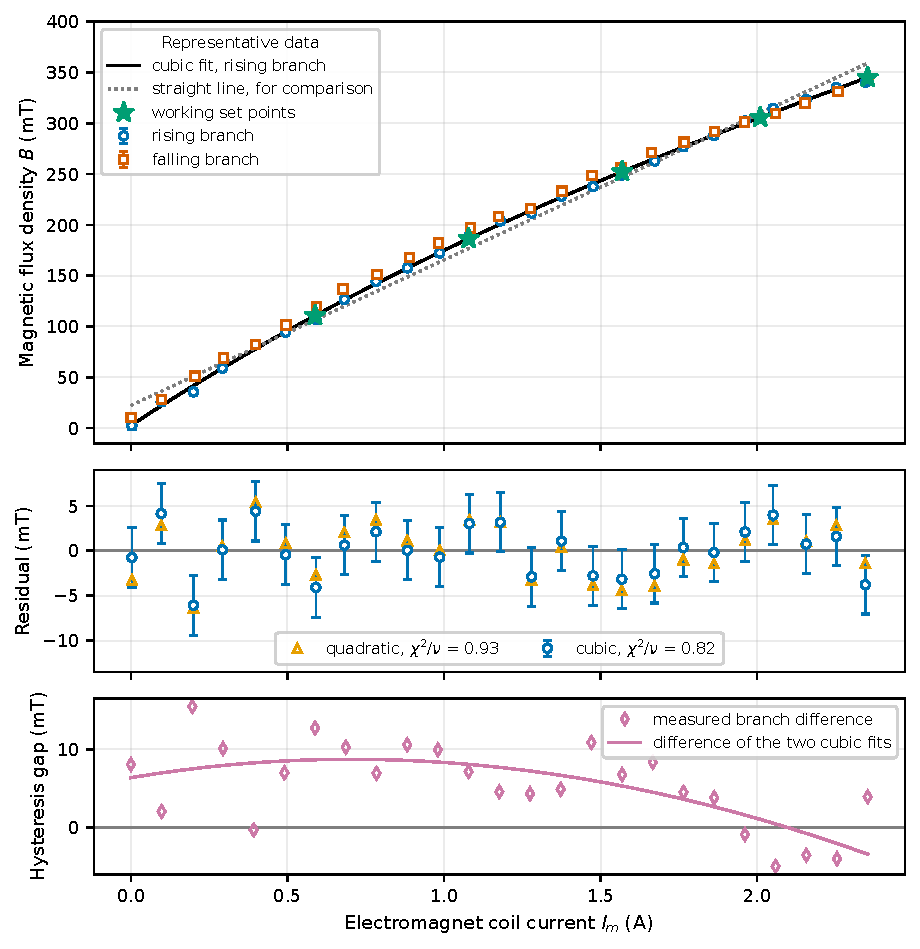
\includegraphics[width=0.62\textwidth]{figures/fig_hall_magnet_calibration.pdf}
\caption{Representative data. Electromagnet calibration against a Hall probe magnetometer.
Top: both hysteresis branches with the cubic fit to the rising branch, a straight line for
comparison, and the five working set points marked. Middle: residuals of the quadratic and
cubic fits. Bottom: the gap between the two branches, measured and from the difference of the
two fitted cubics.}
\label{fig:calibration}
\end{figure}

The five working set points used for every later measurement are listed in
Table~\ref{tab:setpoints}. The peak field of \qty{0.3451}{\tesla} is typical of a
teaching-scale iron-cored electromagnet.

\begin{table}[htbp]
\centering
\caption{Representative data. The five working field settings, with the field from the
rising-branch cubic and the uncertainty on $B$ at each set point. That uncertainty combines
the fit covariance, which alone would give \qtyrange{1.0}{2.3}{\milli\tesla}, with the
branch-reproducibility term and the coil-current reading error folded in through the local
slope. The coil currents are the nominal supply voltage divided by the \qty{10.2}{\ohm} coil
resistance; the measured currents in Appendix~\ref{app:magnet} differ from these by up to
\qty{8}{\milli\ampere}, which shifts the calibrated field by under \qty{1}{\milli\tesla} and
is well inside the quoted uncertainty.}
\label{tab:setpoints}
\begin{tabular}{lrrrrr}
\toprule
Magnet supply (\unit{\volt}) & 6.0 & 11.0 & 16.0 & 20.5 & 24.0 \\
Coil current (\unit{\ampere}) & 0.588 & 1.078 & 1.569 & 2.010 & 2.353 \\
$B$ from the cubic (\unit{\tesla}) & 0.1107 & 0.1864 & 0.2523 & 0.3058 & 0.3451 \\
$\sigma_B$ (\unit{\milli\tesla}) & 2.47 & 2.35 & 2.39 & 2.36 & 3.09 \\
\bottomrule
\end{tabular}
\end{table}

\subsection{The manual familiarisation measurement}
\label{sec:manualresult}

The readings taken by hand in Section~\ref{sec:manual} are in Table~\ref{tab:manual}. They are
not a separate data set. They are four rows lifted out of the same representative arrays that
Appendices~\ref{app:vl} and~\ref{app:vh300} list in full, taken at the top field setting of
\qty{0.3451}{\tesla}, and they are worked here the way they would be worked at the bench: one
point at a time on a calculator, with no fitting and no offset term.

\begin{table}[htbp]
\centering
\caption{Representative data. The manual familiarisation readings, a four-point subset of the
arrays in Appendices~\ref{app:vl} and~\ref{app:vh300}, reduced point by point as
$\Rhtwod = V_H/(IB)$ and $\Rsq = V_L/(3I)$. The two currents differ slightly between the Hall
and longitudinal columns because they come from two separate sweeps at the same bar supply
voltage, one with the magnet on and one with it off.}
\label{tab:manual}
\small
\begin{tabular}{rrrrrrr}
\toprule
Bar supply & \multicolumn{2}{c}{Hall pair, \qty{0.3451}{\tesla}} &
\multicolumn{2}{c}{Longitudinal pair, zero field} & & \\
\cmidrule(lr){2-3}\cmidrule(lr){4-5}
(\unit{\volt}) & $I$ (\unit{\micro\ampere}) & $V_H$ (\unit{\milli\volt})
& $I$ (\unit{\micro\ampere}) & $V_L$ (\unit{\milli\volt})
& $\Rhtwod$ (\unit{\ohm\per\tesla}) & $\Rsq$ (\unit{\ohmsq}) \\
\midrule
3.000  &  9.84 &  4.558 &  9.73 &  46.18 & 1343 & 1583 \\
10.059 & 33.04 & 14.806 & 33.18 & 154.89 & 1299 & 1556 \\
18.529 & 60.87 & 26.897 & 60.66 & 284.37 & 1281 & 1563 \\
27.000 & 88.51 & 39.110 & 88.56 & 415.85 & 1280 & 1565 \\
\midrule
Mean   &       &        &       &        & 1301 & 1567 \\
\bottomrule
\end{tabular}
\end{table}

Averaging the four gives $\Rhtwod = \qty{1301}{\ohm\per\tesla}$ and
$\Rsq = \qty{1567}{\ohmsq}$, and equation~\eqref{eq:mu} then gives

\begin{equation}
\nsq = \frac{1}{e\,\Rhtwod} = \qty{4.8e15}{\per\metre\squared},
\qquad
\mu = \frac{\Rhtwod}{\Rsq} = \qty{0.83}{\metre\squared\per\volt\per\second},
\label{eq:manual}
\end{equation}

quoted to two figures, because two figures is all this method supports. Against the full-array
results of Table~\ref{tab:headline} the density is \num{5.1} per cent low and the mobility
\num{4.9} per cent high.

That error is not random, and it would be wrong to quote the four points as though it were. The
standard error on the mean of the four Hall coefficients is \qty{15}{\ohm\per\tesla}, about
\num{1.1} per cent, but the four values fall steadily from \qty{1343}{\ohm\per\tesla} at the
lowest current to \qty{1280}{\ohm\per\tesla} at the highest, which is a trend and not scatter,
so the standard error on the mean measures nothing real. Section~\ref{sec:reduction} identifies
the trend. Dividing the full model through by $IB$ leaves
$V_H/(IB) = m_H + k/B + c/(IB)$, so a point-by-point ratio carries a bias of $k/B + c/(IB)$, and
at this field setting that bias runs from \qty{124}{\ohm\per\tesla} at the lowest current down
to \qty{51}{\ohm\per\tesla} at the highest, \numrange{10}{4} per cent of the Hall coefficient.
Taking the mean of those four bias terms off the manual average leaves
\qty{1227}{\ohm\per\tesla}, within \num{0.7} per cent of the \qty{1234.9}{\ohm\per\tesla}
adopted later, so the bias accounts for essentially all of the discrepancy.

The longitudinal side behaves much better, and it should: $\Rsq$ from the four points is
\num{0.4} per cent from the fitted value of Section~\ref{sec:rsq300}, because the longitudinal
pair carries no offset term and the measurement has no field in it at all.

The honest summary is that the manual stage gets $\nsq$ and $\mu$ right to about five per cent.
That is enough to confirm the wiring, the polarity and the order of magnitude, which is what it
is for, and it is not enough for anything else. It cannot properly be quoted with an
uncertainty, because four points sharing one systematic give no way to estimate one. Turning it
into a result with a defensible error bar is what the \num{90}-point arrays and the
three-parameter fit of Section~\ref{sec:reduction} are for.

\subsection{Resistance per square at room temperature}
\label{sec:rsq300}

The first objective is answered by a single zero-field sweep. The longitudinal voltage
between contacts 1 and 4 was recorded against sample current with the magnet off; an extract
is given in Table~\ref{tab:vlextract}, the sweep is plotted in Figure~\ref{fig:vl} and the
full \num{18}-point data set is in Appendix~\ref{app:vl}. A weighted straight line
$V_L = m_L I + c_L$ gives $m_L = R_L = \qty{4682.8(61)}{\ohm}$ with an intercept of
\qty{0.36(30)}{\milli\volt}, consistent with zero, and $\chi^2/\nu = 0.95$. Dividing by the
three squares,

\begin{equation}
\Rsq(\qty{300}{\kelvin}) = \frac{m_L}{3} = \qty{1560.9(20)}{\ohmsq}\ \text{(statistical)},
\qquad \qty{1561(16)}{\ohmsq}\ \text{(total)} .
\end{equation}

\begin{table}[htbp]
\centering
\caption{Representative data. Extract from the zero-field longitudinal sweeps at both
temperatures: every third point, together with the last point of the sweep. The complete
tables are in Appendix~\ref{app:vl}.}
\label{tab:vlextract}
\small
\begin{tabular}{rrrrr}
\toprule
Bar supply & \multicolumn{2}{c}{\qty{300}{\kelvin}} & \multicolumn{2}{c}{\qty{79}{\kelvin}} \\
\cmidrule(lr){2-3}\cmidrule(lr){4-5}
(\unit{\volt}) & $I$ (\unit{\micro\ampere}) & $V_L$ (\unit{\milli\volt})
               & $I$ (\unit{\micro\ampere}) & $V_L$ (\unit{\milli\volt}) \\
\midrule
\datarows{tables/tab_VL_extract.tex}
\bottomrule
\end{tabular}
\end{table}

\begin{figure}[htbp]
\centering
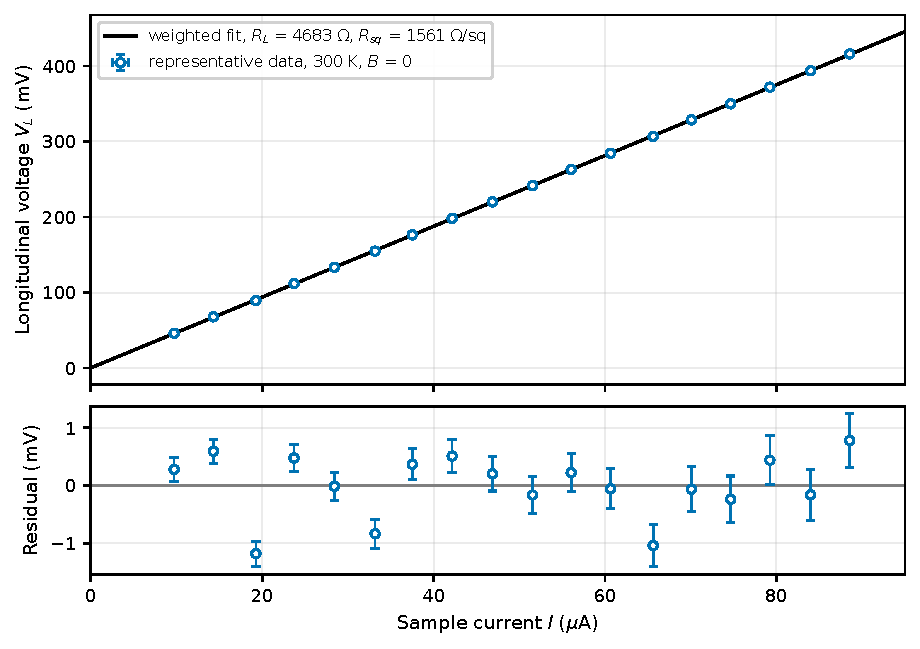
\includegraphics[width=0.74\textwidth]{figures/fig_hall_VL_vs_I.pdf}
\caption{Representative data. Longitudinal voltage against sample current at zero field and
\qty{300}{\kelvin}, with the weighted straight-line fit and its residuals. The fitted slope
is $R_L = \qty{4683}{\ohm}$, giving $\Rsq = \qty{1561}{\ohmsq}$.}
\label{fig:vl}
\end{figure}

\subsection{Dependence of the Hall voltage on current and field}
\label{sec:objective2}

Equation~\eqref{eq:vh2d} makes a sharp prediction: $V_H$ should be a single linear function
of the \emph{product} $IB$, not separately of $I$ and of $B$. The test was made in two
stages. At \qty{300}{\kelvin} the bar supply was swept over \num{18} steps at each of the
five field settings, giving currents from \qtyrange{9.69}{88.75}{\micro\ampere}, Hall
voltages from \qtyrange{1.804}{39.110}{\milli\volt} and products $IB$ from
\qtyrange{1.073}{30.543}{\micro\ampere\tesla}. The cryogenic array covered
\qtyrange{9.71}{90.11}{\micro\ampere}, \qtyrange{1.710}{43.875}{\milli\volt} and
\qtyrange{1.075}{31.033}{\micro\ampere\tesla}. Both full arrays are in
Appendices~\ref{app:vh300} and~\ref{app:vh77}.

The polarity is worth recording, because it is half of the objective. The transverse voltage
on the Hall pair kept one and the same sign at every field setting and every current, and
with the field in the direction marked on the magnet and the current driven from the positive
end contact, that sign is the one equation~\eqref{eq:rh3d} requires for a negative carrier
charge. Conduction is therefore by electrons, as the heterostructure requires. The tabulated
voltages, and every Hall coefficient quoted below, are magnitudes.

A weighted straight line $V_H = s_j I + b_j$ was fitted at each field setting.
Table~\ref{tab:slopes} gives the results at both temperatures and Figure~\ref{fig:vhvsi}
shows the room-temperature family. Every line is straight within the scatter, which answers
the current half of the objective.

\begin{table}[htbp]
\centering
\caption{Representative data. Weighted straight-line fits of $V_H$ against $I$ at each field
setting and at both temperatures. The uncertainties on the intercepts are
\qtyrange{0.029}{0.041}{\milli\volt} throughout. The room-temperature intercepts are all
positive and average \qty{0.27}{\milli\volt}, about four times the cryogenic average of
\qty{0.07}{\milli\volt}, and neither set grows with field. In the model adopted in
Section~\ref{sec:reduction} the intercept at fixed field identifies the current-independent
offset $c$ on the Hall pair, which is distinct from the current-proportional misalignment
term $k$: that term is proportional to $I$ and so is absorbed into the fitted slopes $s_j$,
not into the intercepts.}
\label{tab:slopes}
\small
\begin{tabular}{rrrrrcrrrr}
\toprule
& \multicolumn{4}{c}{\qty{300}{\kelvin}} & & \multicolumn{4}{c}{\qty{79}{\kelvin}} \\
\cmidrule(lr){2-5}\cmidrule(lr){7-10}
$B$ (\unit{\tesla}) & $s_j$ (\unit{\ohm}) & $\sigma_{s_j}$ (\unit{\ohm}) &
$b_j$ (\unit{\milli\volt}) &
$\chi^2/\nu$ & & $s_j$ (\unit{\ohm}) & $\sigma_{s_j}$ (\unit{\ohm}) &
$b_j$ (\unit{\milli\volt}) &
$\chi^2/\nu$ \\
\midrule
0.1107 & 149.8 & 0.5 & $+0.3220$ & 0.95 & & 157.9 & 0.5 & $+0.1080$ & 0.74 \\
0.1864 & 244.8 & 0.6 & $+0.2934$ & 0.71 & & 265.4 & 0.6 & $+0.1519$ & 1.19 \\
0.2523 & 327.3 & 0.7 & $+0.2645$ & 2.17 & & 359.9 & 0.7 & $+0.0639$ & 1.14 \\
0.3058 & 393.9 & 0.7 & $+0.1862$ & 0.51 & & 434.1 & 0.8 & $+0.0481$ & 0.95 \\
0.3451 & 438.9 & 0.8 & $+0.2876$ & 0.92 & & 488.7 & 0.8 & $-0.0108$ & 0.96 \\
\bottomrule
\end{tabular}
\end{table}

\begin{figure}[htbp]
\centering
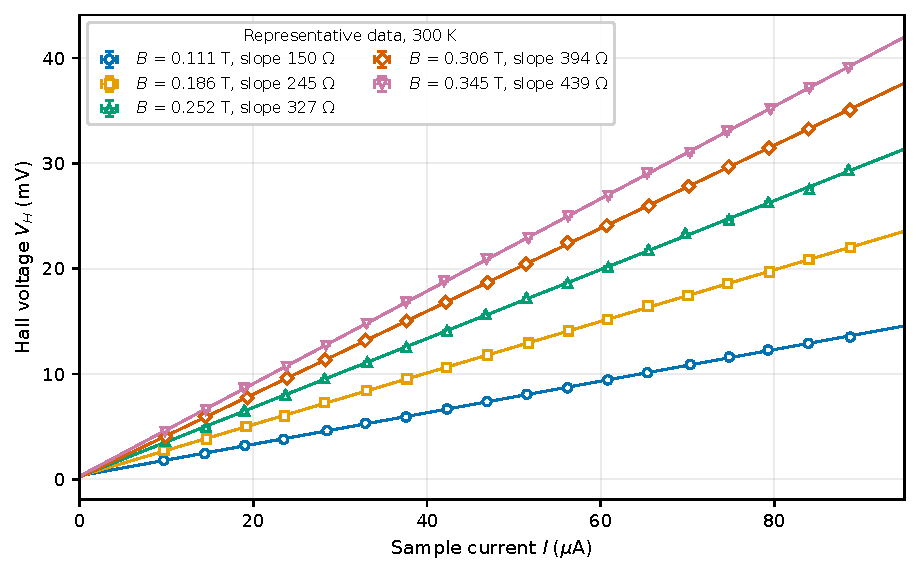
\includegraphics[width=0.78\textwidth]{figures/fig_hall_VH_vs_I.pdf}
\caption{Representative data. Hall voltage against sample current at \qty{300}{\kelvin} for
each of the five calibrated field settings, with the weighted straight-line fit at each
field.}
\label{fig:vhvsi}
\end{figure}

Fitting the five slopes against field as $s(B) = m_H B + k$ gives
$m_H = \qty{1241.0(34)}{\ohm\per\tesla}$ with $k = \qty{13.08(79)}{\ohm}$ at
\qty{300}{\kelvin} and $m_H = \qty{1414.3(35)}{\ohm\per\tesla}$ with
$k = \qty{1.75(80)}{\ohm}$ at \qty{79}{\kelvin}. The slopes are linear in $B$, which answers
the field half of the objective. Taken with Table~\ref{tab:slopes}, $V_H$ is shown to be a
single linear function of the product $IB$ rather than of $I$ and $B$ separately. The
$\chi^2/\nu$ of this second-stage fit, \num{5.64} and \num{1.92} on three degrees of freedom,
sits above unity because its weights carry only the statistical error on each slope: the five
field values come from one shared calibration polynomial, so their errors are correlated
rather than independent and are handled in the systematic budget of
Section~\ref{sec:uncertainties} instead of in the weights.

\subsection{Reducing the whole array to one number}
\label{sec:reduction}

The final objective asks for the best way of collapsing \num{90} readings into a single Hall
coefficient with a sensible error. Three reductions were compared, at both temperatures, and
are set out in Table~\ref{tab:reductions}.

\begin{table}[htbp]
\centering
\caption{Representative data. Three reductions of the \num{90}-point Hall arrays. $\Rhtwod$
and its statistical uncertainty are in \unit{\ohm\per\tesla}. R1 has three degrees of
freedom, R2 has \num{88} and R3 has \num{87}. R3 is adopted at both temperatures.}
\label{tab:reductions}
\small
\begin{tabular}{llrrrcrrr}
\toprule
& & \multicolumn{3}{c}{\qty{300}{\kelvin}} & & \multicolumn{3}{c}{\qty{79}{\kelvin}} \\
\cmidrule(lr){3-5}\cmidrule(lr){7-9}
Reduction & Model & $\Rhtwod$ & $\sigma$ stat & $\chi^2/\nu$ & &
$\Rhtwod$ & $\sigma$ stat & $\chi^2/\nu$ \\
\midrule
R1, slope of slopes & $s_j = m_H B_j + k$ & 1241.0 & 3.4 & 5.64 & &
  1414.3 & 3.5 & 1.92 \\
R2, naive global line & $V_H = m_H (IB) + c$ & 1273.8 & 1.0 & 14.20 & &
  1415.8 & 1.1 & 2.41 \\
R3, global with offset & $V_H = m_H (IB) + kI + c$ & \textbf{1234.9} & \textbf{1.5} &
  \textbf{1.51} & & \textbf{1406.4} & \textbf{1.6} & \textbf{1.73} \\
\bottomrule
\end{tabular}
\end{table}

R2 forces the contact-misalignment voltage, which is proportional to $I$ and independent of
$B$, into a single constant. That voltage is correlated with the abscissa $IB$, so it biases
the slope. At room temperature R2 returns \qty{1273.8}{\ohm\per\tesla} against the R3 value
of \qty{1234.9}{\ohm\per\tesla}, a difference of \num{+3.15} per cent, and its $\chi^2/\nu$
of \num{14.20} says plainly that the two-parameter model does not describe the data. The
lower panel of Figure~\ref{fig:collapse} shows why: the R2 residuals are grouped into visible
bands by field setting and that structure is largely gone once the $kI$ term is added. The
weighted residual RMS falls from \qty{0.2421}{\milli\volt} to \qty{0.0853}{\milli\volt}.

R1 and R3 agree to \num{+0.49} per cent at room temperature and \num{+0.56} per cent cold, so
little turns on the choice between them. R3 is preferred because it uses every point in one
weighted fit rather than fitting slopes to slopes, and because it returns the offset as an
explicit parameter. A fourth possibility, computing $\Rhtwod = V_H/(IB)$ point by point and
taking the mean, is worse than any of the three. Dividing the full model through by $IB$
gives $V_H/(IB) = m_H + k/B + c/(IB)$, so the ratio carries two spurious terms rather than
one. It weights the smallest $IB$ points, which have the worst signal-to-noise ratio, equally
with the best, and the constant offset contributes $c/(IB)$ to every ratio, a contribution
that diverges as $IB$ goes to zero; the misalignment term contributes a further $k/B$ to every
ratio, and that one does not fall away as the current is raised. At the lowest field setting
it is \qty{130}{\ohm\per\tesla}, about \num{10} per cent of the Hall coefficient itself. That
unweighted average returns \qty{1346.2}{\ohm\per\tesla} at room temperature, \num{9.0} per
cent from the adopted value, and \qty{1436.3}{\ohm\per\tesla} cold, \num{2.1} per cent away.

\begin{figure}[htbp]
\centering
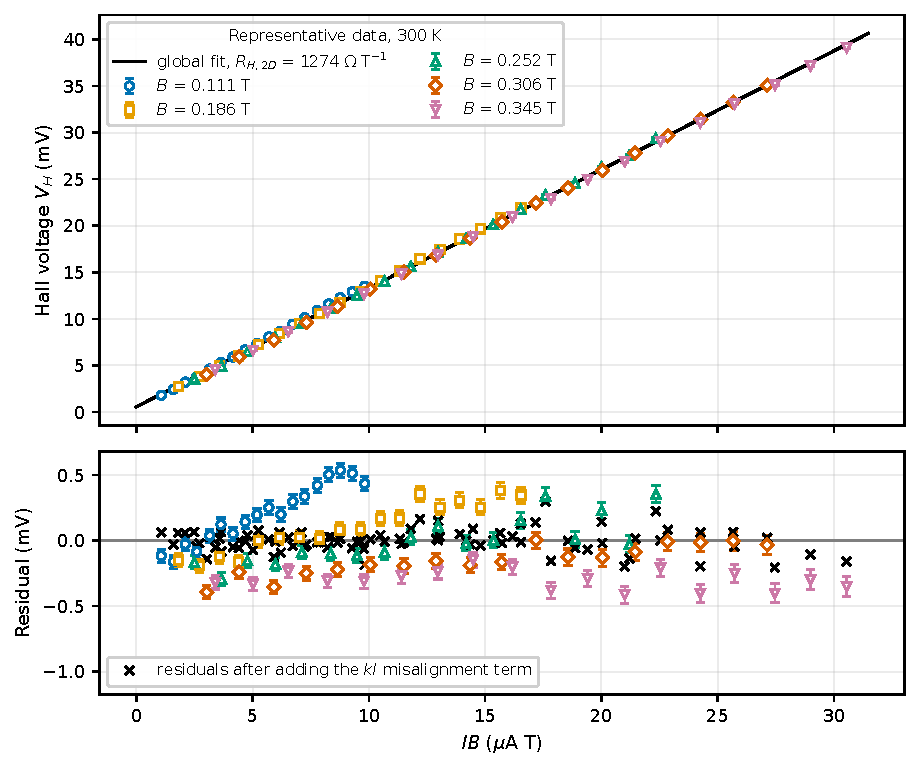
\includegraphics[width=0.76\textwidth]{figures/fig_hall_VH_vs_IB.pdf}
\caption{Representative data. Top: all \num{90} room-temperature Hall readings collapsed onto
the product $IB$, with the naive two-parameter global fit drawn through them. Bottom:
residuals of that fit coloured by field setting, together with the residuals of the
three-parameter fit as black crosses. The banding by field setting in the first set, and its
absence in the second, is the evidence for the contact-misalignment term.}
\label{fig:collapse}
\end{figure}

The nuisance parameters returned by R3 are $k = \qty{14.41(43)}{\ohm}$ with
$c = \qty{+0.277(15)}{\milli\volt}$ at room temperature, and $k = \qty{3.44(44)}{\ohm}$
with $c = \qty{+0.084(15)}{\milli\volt}$ cold. The fitted $c$ matches the mean per-field
intercept of Table~\ref{tab:slopes} at both temperatures, \qty{0.271}{\milli\volt} and
\qty{0.072}{\milli\volt}, which is exactly what this model requires: at fixed $B$ the $kI$
term is proportional to $I$ and so lands in the slope, leaving $c$ alone in the intercept. The quoted standard error on $k$ understates how well it is really known, because
$k$ is strongly correlated with $m_H$: the correlation coefficient from the covariance matrix
is $-0.75$ at room temperature and $-0.74$ cold. Any error in the field calibration therefore
leaks into $k$ as well as into the slope, and $k$ should be read as a parameter that soaks up
a field-independent voltage rather than as a precision measurement of the contact geometry.

The objective asks for the density and the mobility, not only for $\Rhtwod$, so it is worth
saying what each reduction would give. At \qty{300}{\kelvin} R1, R2 and R3 give
$\nsq = \num{5.03}$, \num{4.90} and \qty{5.05e15}{\per\metre\squared} with
$\mu = \num{0.795}$, \num{0.816} and
\qty{0.791}{\metre\squared\per\volt\per\second}; cold they give $\nsq = \num{4.41}$,
\num{4.41} and \qty{4.44e15}{\per\metre\squared} with $\mu = \num{12.00}$, \num{12.01} and
\qty{11.93}{\metre\squared\per\volt\per\second}. The total uncertainty is \num{3.9} per cent
on $\nsq$ and \num{4.0} per cent on $\mu$ whichever reduction is used, since it is dominated
by the magnet calibration and not by the fit, so the choice matters only through the
\num{3.15} per cent bias that R2 carries at room temperature. No comparable choice arises on
the longitudinal side: that is one zero-field sweep with no nuisance parameter in it, so
$m_L$ enters $\mu$ unambiguously.

\subsection{Angular dependence of the Hall voltage}
\label{sec:angle}

The angular scan was taken at \qty{300}{\kelvin} with the magnet supply fixed at
\qty{20.5}{\volt}, a calibrated field of \qty{0.3058}{\tesla}, and the bar supply fixed at
\qty{18.3}{\volt}, giving a mean sample current of \qty{60.07}{\micro\ampere}. The rotation
stage was stepped through a full \ang{360} in \ang{15} steps; the data are in
Appendix~\ref{app:angle} and Figure~\ref{fig:angle}. Fitting equation~\eqref{eq:angle} by
weighted least squares gave

\begin{equation}
V_{H0} = \qty{22.855(16)}{\milli\volt}, \qquad
\theta_0 = \qty{6.07(4)}{\degree}, \qquad
C = \qty{1.002(11)}{\milli\volt},
\label{eq:anglefit}
\end{equation}

with $\chi^2 = 28.34$ on \num{22} degrees of freedom, $\chi^2/\nu = 1.29$, and an RMS
residual of \qty{0.0582}{\milli\volt} against an assumed meter scatter of
\qty{0.050}{\milli\volt}. The excess above unity has an obvious source. The fit holds
$V_{H0}$ constant, but the sample current was not perfectly constant across the scan: it
ranged from \qtyrange{59.92}{60.44}{\micro\ampere}, a standard deviation of \num{0.2} per
cent, which is about \qty{0.05}{\milli\volt} near the peak and so is comparable with the
residual itself.

The uncertainties in equation~\eqref{eq:anglefit} are the fit standard errors, and the fit
weights $V_H$ alone. Section~\ref{sec:angleuncert} adds the uncertainty of setting the angle
itself. It leaves $V_{H0}$ and $C$ untouched but widens $\theta_0$ to
\qty{6.07(8)}{\degree}, and that is the figure quoted elsewhere in this report.

\begin{figure}[htbp]
\centering
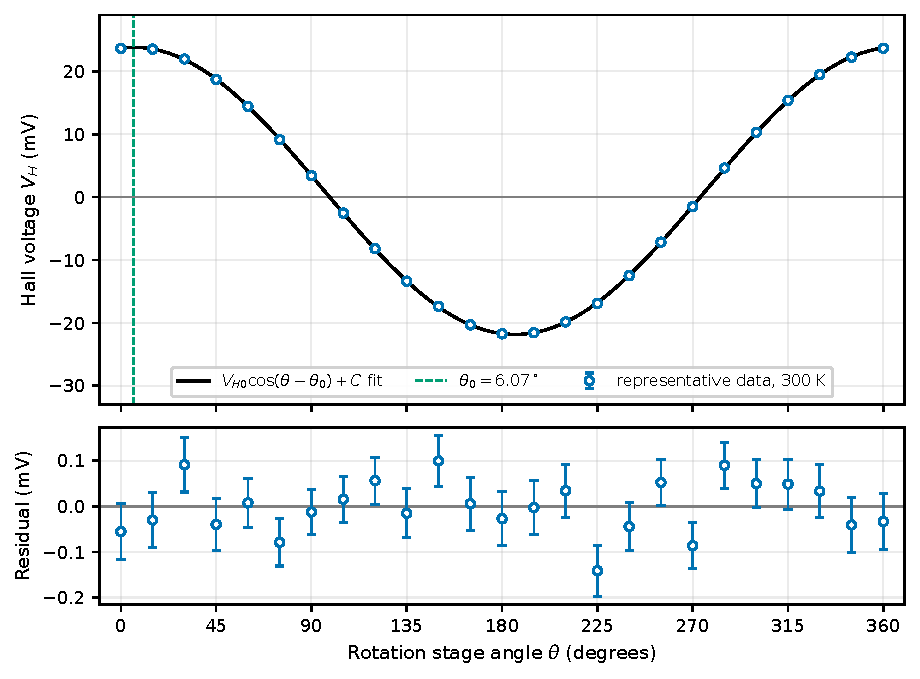
\includegraphics[width=0.76\textwidth]{figures/fig_hall_angle.pdf}
\caption{Representative data. Hall voltage against rotation stage angle over a full \ang{360}
at \qty{300}{\kelvin}, at fixed field \qty{0.3058}{\tesla} and fixed mean current
\qty{60.07}{\micro\ampere}, with the fitted cosine and its residuals. The fitted misalignment
$\theta_0 = \ang{6.07}$ is marked.}
\label{fig:angle}
\end{figure}

Four things follow. First, the scan is a check on the Hall coefficient: the amplitude
predicted from the separately fitted $\Rhtwod$ and the measured $I$ and $B$ is
\qty{22.69}{\milli\volt} against a fitted \qty{22.855}{\milli\volt}, a difference of
\num{+0.75} per cent. That difference should not be measured against the \num{3.9} per cent
magnet systematic, because the prediction multiplies $\Rhtwod$ by the same calibrated field
that was used to obtain $\Rhtwod$ in the first place, so a scale error in $B$ cancels between
the two determinations and the comparison tests the shape of the calibration polynomial at one
set point rather than its scale. Against the statistical errors that do apply, \num{0.07} per
cent on the fitted amplitude and about \num{0.12} per cent on the prediction through $m_H$ and
the mean current, \num{0.15} per cent combined, the difference is about five standard errors.
The likely causes are the local error of the cubic at this one set point, drift of the current
noted above, and the fact that the offset absorbed by the two fits is not the same quantity.
The check still bounds any gross error in $\Rhtwod$ below one per cent.

Second, $\theta_0$ is a mounting misalignment between the zero of the rotation stage and the
orientation in which the sample normal is truly parallel to the field, with contributions
from the angular scale zero, from how the plug-in box seats in its holder and from the chip
not being mounted perfectly flat. It says nothing about the sample, and because the cosine is
flat near its maximum a measurement taken at a nominal zero under-reads the normal field
component by only \num{0.56} per cent. Third, the offset $C = \qty{1.002}{\milli\volt}$ is
field-independent and is close in size to the offset found independently in the global fit,
which predicts $kI + c = \qty{1.143}{\milli\volt}$ at this current, made up of
\qty{0.866}{\milli\volt} from $kI$ and \qty{0.277}{\milli\volt} from $c$. The two differ by
\num{-12.3} per cent, which is about four standard errors once the \qty{0.030}{\milli\volt} on
$kI + c$ and the \qty{0.011}{\milli\volt} on $C$ are combined, so they are not the same
quantity within their fitted precision. The angular scan measures the offset at one current
and one field setting, while $k$ and $c$ are averaged over the whole \num{90}-point array and
$k$ correlates with the slope at $-0.75$. Taken with the temperature dependence of $k$ in
Section~\ref{sec:rtharder}, the reading that fits both observations is that a second
field-independent term is present which the two-term model $kI + c$ does not fully capture.

Fourth, the fitted cosine term reverses sign at $\theta_0 + \ang{180}$ with equal magnitude
while the constant $C$ does not, so the measured voltage does not. The readings at
\ang{0} and \ang{180} are \qty{+23.674}{\milli\volt} and \qty{-21.752}{\milli\volt}: they
differ in magnitude by \qty{1.92}{\milli\volt}, which is $2C$ within the scatter, an asymmetry
of \num{8.5} per cent. That asymmetry is itself the signature of the offset. Taking half the
difference of two opposite angles,
$\tfrac12\left[V_H(\theta)-V_H(\theta+\ang{180})\right] = \qty{22.713}{\milli\volt}$, removes
$C$ exactly and returns the pure Hall term, while half their sum,
\qty{0.961}{\milli\volt}, returns $C$ and so measures the offset a second, independent way.
This is the same odd-in-$B$, even-in-$B$ argument as reversing the field in
Section~\ref{sec:improvements}, and the reversal itself confirms that the signal is a genuine
Hall voltage rather than an instrumental artefact.

\subsection{Cryogenic run and summary of results}
\label{sec:results77}

The type K thermocouple readings taken through the cold run, listed in
Appendix~\ref{app:thermo}, have a mean of
\qty{78.69}{\kelvin}, a standard deviation of \qty{1.11}{\kelvin} and a standard error on the
mean of \qty{0.32}{\kelvin}. The accuracy floor of a type K junction below
\qty{200}{\kelvin} is about \qty{2.5}{\kelvin} and dominates, so the temperature is quoted as
$T = \qty{79(3)}{\kelvin}$. That is a few kelvin above the liquid nitrogen boiling point of
\qty{77.4}{\kelvin} at one atmosphere, which is expected: the bead is on the mount rather
than on the 2DEG, and the sample sits above the liquid in a pumped dewar. The sensitivity of
a type K junction falls from about \qty{41}{\micro\volt\per\kelvin} at \qty{300}{\kelvin} to
roughly \qty{16}{\micro\volt\per\kelvin} at \qty{77}{\kelvin}, which is why the cold reading
is the less precise one. Neither $\nsq$ nor $\mu$ is calculated from $T$, so this uncertainty
does not propagate into the results; it matters only for comparison with literature values
quoted at a nominal \qty{77}{\kelvin}.

The zero-field longitudinal sweep at this temperature gave
$m_L = R_L = \qty{353.63(69)}{\ohm}$ with an intercept of \qty{0.111(35)}{\milli\volt} and
$\chi^2/\nu = 0.78$, so $\Rsq = \qty{117.88(23)}{\ohmsq}$ statistical and
\qty{117.9(12)}{\ohmsq} in total. Applying equation~\eqref{eq:working} at both temperatures
gives the results collected in Table~\ref{tab:headline}. Figure~\ref{fig:comparison} places
the two temperatures side by side.

\begin{table}[htbp]
\centering
\caption{Representative data. Headline results. $\Rhtwod$ comes from the R3 global weighted
fit and $\Rsq$ from the zero-field longitudinal fit. Note that
\qty{e15}{\per\metre\squared} is exactly \qty{e11}{\per\centi\metre\squared}, so the density
carries the same digits in the units the literature usually quotes. The mobility in those
units is \qty{7910(320)}{\centi\metre\squared\per\volt\per\second}, the figure carried into
Table~\ref{tab:literature}, and
\qty{119300(4800)}{\centi\metre\squared\per\volt\per\second}. The product $\nsq\mu$ is
equivalently $1/(e\Rsq)$, in \unit{\per\coulomb\per\ohm}. The two ratios between the
temperatures, and the changes on cooling, carry statistical uncertainties only: both columns
were measured with one field calibration and one value of $l/w$, so the magnet and geometry
systematics are common to them and cancel in any ratio between them.}
\label{tab:headline}
\begin{tabular}{lrrl}
\toprule
Quantity & \qty{300}{\kelvin} & \qty{79(3)}{\kelvin} & Change on cooling \\
\midrule
$\Rhtwod$, statistical only (\unit{\ohm\per\tesla}) & $1234.9 \pm 1.5$ & $1406.4 \pm 1.6$ & \\
$\Rhtwod$, total (\unit{\ohm\per\tesla}) & $1235 \pm 48$ & $1406 \pm 54$ &
  $+13.9$ per cent \\
$R_L$ (\unit{\ohm}) & $4682.8 \pm 6.1$ & $353.63 \pm 0.69$ & \\
$\Rsq$, total (\unit{\ohmsq}) & $1561 \pm 16$ & $117.9 \pm 1.2$ &
  factor 13.2 decrease \\
$\nsq$, total (\qty{e15}{\per\metre\squared}) & $5.05 \pm 0.20$ & $4.44 \pm 0.17$ &
  $-12.2$ per cent \\
$\nsq$, statistical only & $5.054 \pm 0.006$ & $4.438 \pm 0.005$ & \\
$\nsq(\qty{79}{\kelvin})/\nsq(\qty{300}{\kelvin})$ &
  \multicolumn{2}{c}{$0.8781 \pm 0.0015$} & systematics cancel \\
$\mu$, total (\unit{\metre\squared\per\volt\per\second}) & $0.791 \pm 0.032$ &
  $11.93 \pm 0.48$ & factor $15.08 \pm 0.04$ \\
$\mu$, statistical only & $0.7912 \pm 0.0014$ & $11.93 \pm 0.03$ & \\
$\nsq\mu$ (\qty{e15}{\per\volt\per\second}) & $3.999 \pm 0.040$ &
  $52.95 \pm 0.54$ & free of magnet error \\
\bottomrule
\end{tabular}
\end{table}

\begin{figure}[htbp]
\centering
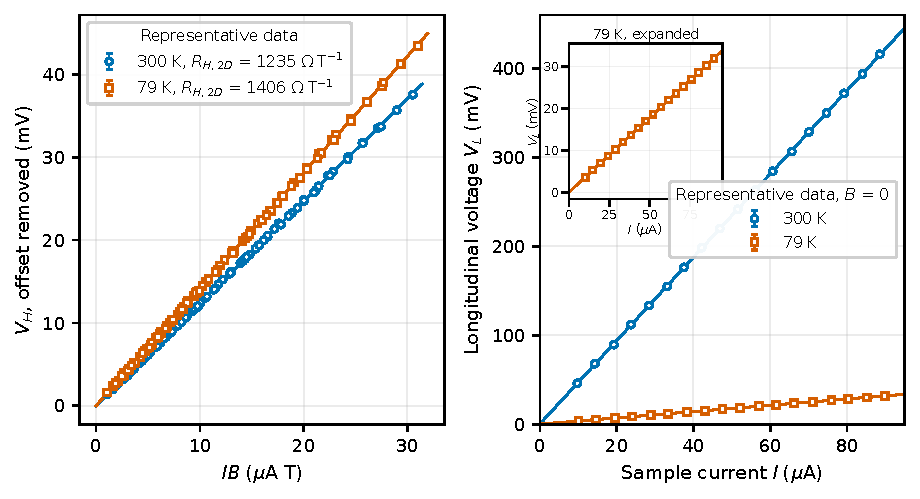
\includegraphics[width=0.88\textwidth]{figures/fig_hall_77K_comparison.pdf}
\caption{Representative data. Left: Hall voltage against $IB$ at both temperatures with the
fitted misalignment term $kI$ and the constant $c$ subtracted, so the remaining signal is the
pure Hall term and the fitted lines pass through the origin. Right: raw zero-field
longitudinal voltages at both temperatures, with the cryogenic data repeated in an expanded
inset.}
\label{fig:comparison}
\end{figure}

\subsection{Secondary quantities}
\label{sec:secondary}

Several further quantities follow with no extra measurement, taking the electron effective
mass in the GaAs conduction band as $m^{*} = 0.067\,m_0$~\cite{vurgaftman2001}. They are
collected in Table~\ref{tab:secondary} because the discussion needs them.

The first of them, the momentum relaxation time $\tau$, needs a line of derivation, because it
does not follow from anything written down so far. In the Drude picture a carrier is
accelerated by the applied field and loses its drift momentum on average once every $\tau$, so
in the steady state the momentum gained between collisions balances the momentum lost.
Writing magnitudes, as everywhere in this report,

\begin{equation}
\frac{m^{*} v_d}{\tau} = eE
\quad\Longrightarrow\quad
\mu \equiv \frac{v_d}{E} = \frac{e\tau}{m^{*}}
\quad\Longrightarrow\quad
\tau = \frac{\mu\,m^{*}}{e}.
\label{eq:tau}
\end{equation}

The mobilities of Table~\ref{tab:headline} therefore give $\tau = \qty{0.301}{\pico\second}$ at
\qty{300}{\kelvin} and \qty{4.55}{\pico\second} at \qty{79}{\kelvin}. It is $\tau$ that then
carries into the mean free path $\ell = v_F\tau$ and into the product $\omega_c\tau = \mu B$ in
the rows below, both of which the discussion uses.

\begin{table}[htbp]
\centering
\caption{Representative data. Secondary quantities derived from the fitted sheet density and
mobility, computed with $m^{*} = 0.067\,m_0$. The Fermi quantities are zero-temperature
expressions. At \qty{300}{\kelvin} the gas is not degenerate, $T/T_F = 1.43$, so the
room-temperature entries in the $E_F$, $k_F$, $v_F$ and mean free path rows are indicative
only: using the thermal velocity $\sqrt{2k_BT/m^{*}} = \qty{3.7e5}{\metre\per\second}$ in place
of $v_F$ changes the room-temperature mean free path to \qty{0.11}{\micro\metre} and does not
affect the conclusion that transport is diffusive. In particular the room-temperature $E_F$ is
a degeneracy scale and not the chemical potential, which is \qty{+0.28}{\milli\electronvolt}
there; $T_F$ is defined from $E_F$ and is used in this report only to say how far from
degeneracy the gas is. At \qty{79}{\kelvin} the chemical potential is
\qty{15.16}{\milli\electronvolt} against $E_F = \qty{15.86}{\milli\electronvolt}$, so the two
are close and the zero-temperature expressions are nearly right.}
\label{tab:secondary}
\small
\begin{tabular}{llrrl}
\toprule
Quantity & Formula & \qty{300}{\kelvin} & \qty{79}{\kelvin} & Unit \\
\midrule
Momentum relaxation time $\tau$ & $\mu m^{*}/e$ & 0.301 & 4.55 & \unit{\pico\second} \\
Fermi wavevector $k_F$ & $\sqrt{2\pi \nsq}$ & 1.782 & 1.670 & \qty{e8}{\per\metre} \\
Fermi velocity $v_F$ & $\hbar k_F/m^{*}$ & 3.079 & 2.885 & \qty{e5}{\metre\per\second} \\
Mean free path $\ell$ & $v_F \tau$ & 0.093 & 1.311 & \unit{\micro\metre} \\
Fermi energy $E_F$ & $\pi\hbar^2 \nsq/m^{*}$ & 18.06 & 15.86 & \unit{\milli\electronvolt} \\
Fermi temperature $T_F$ & $E_F/k_B$ & 210 & 184 & \unit{\kelvin} \\
$\omega_c\tau$ at \qty{0.345}{\tesla} & $\mu B$ & 0.273 & 4.12 & dimensionless \\
Density of states $g_{\mathrm{2D}}$ & $m^{*}/\pi\hbar^2$ & 2.799 & 2.799 &
  \qty{e13}{\per\electronvolt\per\centi\metre\squared} \\
\bottomrule
\end{tabular}
\end{table}

\section{Uncertainties}
\label{sec:uncertainties}

\subsection{Random contributions and how the fits were weighted}

The random scatter on a single reading is set by the resolution and accuracy of the bench
multimeters, by Johnson noise in the sample and leads, by mains pickup on unshielded banana
leads, and by slow drift of thermal electromotive forces. The values assigned were a floor of
\qty{0.05}{\milli\volt} on $V_H$ with \num{0.15} per cent of reading in quadrature, a floor
of \qty{0.20}{\milli\volt} on $V_L$ at room temperature with \num{0.10} per cent of reading,
a floor of \qty{0.05}{\milli\volt} on $V_L$ at \qty{79}{\kelvin} with \num{0.15} per cent of
reading, and \qty{0.10}{\micro\ampere} on $I$ with \num{0.10} per cent of reading. In
relative terms the cryogenic longitudinal measurement is the hardest, because $V_L$ there is
only a few tens of millivolts.

Every fit was weighted by $1/\sigma_i^2$ with the abscissa uncertainty folded in through the
local slope, so that for the Hall fits
$\sigma_i^2 = \sigma_{V_H}^2 + (m_H\,\sigma_{(IB),i})^2$. The magnet calibration uncertainty
was deliberately excluded from the weights. It is one correlated systematic shared by every
point taken at a given field setting, not an independent random error on each point, and
treating it as random would both mis-weight the fit and understate the final uncertainty. It
is carried into the budget below instead. This is why a $\chi^2/\nu$ of exactly one is not
expected for the global Hall fits, and why the adopted R3 values sit at \num{1.51} and
\num{1.73}.

\subsection{The angle setting in the angular scan}
\label{sec:angleuncert}

The list above assigns a scatter to every reading the fits weight. The angular scan of
Section~\ref{sec:angle} has a second measured quantity which the fit does not weight at all:
the angle itself. The rotation stage was set and read to the nearest degree, which is the
resolution at which the scan is recorded in Appendix~\ref{app:angle}. Treating that as a
rectangular distribution of half width \ang{0.5} gives a standard uncertainty of
$\sigma_\theta = \ang{0.5}/\sqrt{3} = \ang{0.29}$, or \qty{5.0e-3}{\radian}.

Where that matters follows from the derivative of the fitted cosine,

\begin{equation}
\frac{\mathrm{d}V_H}{\mathrm{d}\theta} = -V_{H0}\sin(\theta-\theta_0),
\label{eq:angderiv}
\end{equation}

which vanishes at the peak. Near $\theta = \theta_0$ the effect is therefore second order,
$\Delta V_H \simeq \tfrac12 V_{H0}(\Delta\theta)^2$, which for $\sigma_\theta$ is
\qty{0.29}{\micro\volt}, a fraction \num{1.3e-5} of the amplitude. On the flanks, where
$\left|\sin(\theta-\theta_0)\right| = 1$, it is first order and much larger:
$V_{H0}\sigma_\theta = \qty{0.115}{\milli\volt}$, about twice the assigned meter scatter of
\qtyrange{0.050}{0.061}{\milli\volt}. The two are equal where
$\left|\sin(\theta-\theta_0)\right| = 0.48$, about \ang{29} either side of the peak and of the
trough, so over most of a full turn it is the angle and not the voltmeter that limits the
reading.

Three things follow, and the first two of them are that it does not matter.

It does not touch $V_{H0}$, which is the only quantity from this scan that any other result
depends on. The amplitude is a peak value, the effect there is second order, and
\num{1.3e-5} is four orders of magnitude below the \num{3.9} per cent magnet systematic. The
\num{0.75} per cent cross-check of the Hall coefficient in Section~\ref{sec:angle} is
therefore unaffected, and so is the \num{0.56} per cent under-reading quoted there for a
measurement taken at a nominal zero.

A common error in the zero of the angular scale does not matter either, and for a sharper
reason: it is exactly degenerate with $\theta_0$. Adding the same offset to every recorded
angle shifts the fitted $\theta_0$ by that offset and leaves $V_{H0}$ and $C$ numerically
unchanged. That is the same statement as the one made in Section~\ref{sec:angle}, that
$\theta_0$ absorbs the angular scale zero along with the mounting, and it is why no systematic
on the scale zero appears in the budget below.

What does matter is the random part of the setting error, and it matters for $\theta_0$
itself. A per-point scatter of \ang{0.29} over \num{25} points gives
$\sigma_\theta/\sqrt{N} = \ang{0.06}$, which in quadrature with the \ang{0.04} fit error is
\ang{0.07}. Refitting the scan with the angle term folded into the weights, so that
$\sigma_i^2 = \sigma_{V_H}^2 + \left(V_{H0}\sin(\theta_i-\theta_0)\,\sigma_\theta\right)^2$,
gives \ang{0.08} directly, and the larger of the two is adopted:
$\theta_0 = \qty{6.07(8)}{\degree}$. That refit is used to size the uncertainty and not to
replace the fitted value; it moves $\theta_0$ by \ang{0.03}, well inside the widened error.
The \ang{0.04} of equation~\eqref{eq:anglefit} is therefore about twice as precise as the
stage can justify.

One caution against pushing this any further. Folding the full \ang{0.29} into the weights
drops $\chi^2/\nu$ from \num{1.29} to \num{0.44}, which says that the scan does not in fact
scatter by that much, and that setting a stage against marked graduations is more repeatable
than the reading resolution on its own suggests. The true per-point angular scatter is
somewhere below \ang{0.29}, so \qty{6.07(8)}{\degree} is a conservative statement rather than a
tight one.

\subsection{Propagation}

For a quantity $f(x_1,\dots,x_N)$ formed from independent measured
quantities~\cite{taylor1997},

\begin{equation}
\sigma_f^2 = \sum_{i=1}^{N}\left(\frac{\partial f}{\partial x_i}\right)^2 \sigma_{x_i}^2 .
\label{eq:prop}
\end{equation}

From $\nsq = 1/(e m_H)$, $\partial \nsq/\partial m_H = -1/(e m_H^2)$, so the fractional
uncertainties are equal in magnitude and

\begin{equation}
\frac{\sigma_{\nsq}}{\nsq} = \sqrt{
\left(\frac{\sigma_{m_H}}{m_H}\right)^2 +
\left(\frac{\sigma_B}{B}\right)^2_{\mathrm{syst}} } .
\label{eq:propn}
\end{equation}

The field term appears because $B$ enters the abscissa of every point in the fit, so a
fractional error in the calibration produces the same fractional error in the slope. From
$\Rsq = m_L/(l/w)$ and $\mu = (l/w)\,m_H/m_L$, both of which carry the geometry through the
ratio $l/w$,

\begin{align}
\frac{\sigma_{\Rsq}}{\Rsq} &= \sqrt{
\left(\frac{\sigma_{m_L}}{m_L}\right)^2 +
\left(\frac{\sigma_l}{l}\right)^2 +
\left(\frac{\sigma_w}{w}\right)^2 } ,
\label{eq:proprsq}\\[2pt]
\frac{\sigma_{\mu}}{\mu} &= \sqrt{
\left(\frac{\sigma_{m_H}}{m_H}\right)^2 +
\left(\frac{\sigma_{m_L}}{m_L}\right)^2 +
\left(\frac{\sigma_l}{l}\right)^2 +
\left(\frac{\sigma_w}{w}\right)^2 +
\left(\frac{\sigma_B}{B}\right)^2_{\mathrm{syst}} } .
\label{eq:propmu}
\end{align}

$\Rsq$ carries no magnet term at all, because it was measured at zero field, and $\nsq$
carries no geometry term at all, for the reason given after equation~\eqref{eq:vh2d}.

\subsection{Systematic contributions}

The magnet calibration is by far the largest systematic, and the three terms that make it up
have to be kept distinct so that nothing is counted twice. The Hall probe magnetometer has an
absolute accuracy of a few per cent, and the probe and the sample do not occupy exactly the
same point in a gap where the field is not perfectly uniform; these were combined as
\num{3.0} per cent. The uncertainty on the calibrated field at a set point, listed in
Table~\ref{tab:setpoints}, is \num{1.2} per cent of $B$ on average; that term already carries
the scatter of the calibration points about the cubic, through the fit covariance, together
with the branch reproducibility and the coil-current reading. A floor term of
\qty{5}{\milli\tesla}, which is \num{2.1} per cent over the mean working field of
\qty{0.240}{\tesla}, covers what the calibration cannot see at all: the branch offset between
the rising-branch calibration and the state the core is actually left in by the measurement
protocol of Section~\ref{sec:calibration}, measured as \qty{5.52}{\milli\tesla} on average and
\qty{6.35}{\milli\tesla} extrapolated to zero coil current, together with any drift of the
magnet between the calibration sweep and the measurement runs. The scatter about the cubic is not repeated
here.

The geometrical systematic enters only through $l/w$. The mask dimensions are disturbed by
lithography and etch bias, typically well under a micrometre, and by lateral depletion at the
etched mesa edge, where surface states pin the Fermi level at the exposed sidewall and
deplete the 2DEG over a few tenths of a micrometre on each side. Together these were assigned
\num{1.0} per cent. The full budget is in Table~\ref{tab:budget}.

\begin{table}[htbp]
\centering
\caption{Representative data. Uncertainty budget. The magnet calibration dominates everything
that depends on the Hall coefficient, and improving the voltmeters would not change the
result. The three magnet terms are kept distinct so that nothing is counted twice: the
scatter of the calibration points about the cubic and the branch reproducibility sit in the
\num{1.2} per cent line, the branch offset between calibration and measurement sits in the
floor term, and neither appears in both. The angle-setting term is listed separately below the
rule because it reaches nothing in the columns above it: it is second order at the peak, so it
does not touch $V_{H0}$, $\nsq$, $\Rsq$ or $\mu$, and a common scale zero error is absorbed
into $\theta_0$ by construction. The per-point setting scatter alone would put \ang{0.06} on
$\theta_0$; refitting with the angle folded into the weights gives \ang{0.08}, and that is the
figure listed here and quoted throughout. Section~\ref{sec:angleuncert} works it through.}
\label{tab:budget}
\small
\begin{tabular}{p{0.56\textwidth}ll}
\toprule
Contribution & Size & Affects \\
\midrule
Fit standard error on $m_H$, \qty{300}{\kelvin} / \qty{79}{\kelvin} &
  0.13 / 0.11 per cent & $\nsq$, $\mu$ \\
Fit standard error on $m_L$, \qty{300}{\kelvin} / \qty{79}{\kelvin} &
  0.13 / 0.19 per cent & $\Rsq$, $\mu$ \\
Hall probe absolute accuracy and positioning in the gap & 3.0 per cent & $\nsq$, $\mu$ \\
Floor term, \qty{5}{\milli\tesla} over a mean field of \qty{0.240}{\tesla}: branch
  offset and magnet drift & 2.1 per cent & $\nsq$, $\mu$ \\
Calibrated field at a set point: fit covariance, branch reproducibility and
  coil-current reading & 1.2 per cent & $\nsq$, $\mu$ \\
\midrule
\textbf{Combined magnet systematic on $B$} & \textbf{3.9 per cent} &
  $\nsq$, $\mu$, not $\Rsq$ \\
Geometry, $l/w$ from etch bias and mesa edge depletion & 1.0 per cent &
  $\Rsq$, $\mu$, not $\nsq$ \\
\midrule
\textbf{Combined on $\nsq$} & \textbf{3.9 per cent} & both temperatures \\
\textbf{Combined on $\Rsq$} & \textbf{1.0 per cent} & both temperatures \\
\textbf{Combined on $\mu$} & \textbf{4.0 per cent} & both temperatures \\
\midrule
Rotation stage set and read to \ang{1}, $\sigma_\theta = \ang{0.29}$: second order at the
  peak, first order on the flanks & \ang{0.08} on $\theta_0$ & $\theta_0$ only \\
\bottomrule
\end{tabular}
\end{table}

\subsection{Correlations, and the quantities that escape the systematic}
\label{sec:correlations}

$\nsq$ and $\mu$ both contain $m_H$, so their errors are correlated rather than independent.
In the product they cancel exactly:

\begin{equation}
\nsq\,\mu = \frac{1}{e\,\Rhtwod}\cdot\frac{\Rhtwod}{\Rsq} = \frac{1}{e\,\Rsq} .
\label{eq:product}
\end{equation}

The product is therefore fixed by the zero-field longitudinal measurement alone and is
completely immune to the magnet calibration. It is known to \num{1.0} per cent at both
temperatures, far better than either factor separately, which is why it is quoted as a line
of its own in Table~\ref{tab:headline}.

Any ratio between the two temperatures escapes the same systematics, and for the same reason.
Both mobilities are built from the same calibration polynomial and the same $l/w$, so those
factors cancel identically in $\mu(\qty{79}{\kelvin})/\mu(\qty{300}{\kelvin})$, leaving only
the four fit standard errors of Table~\ref{tab:budget}, \num{0.29} per cent in quadrature,
hence $15.08 \pm 0.04$. The density ratio behaves the same way: it is
$\Rhtwod(\qty{300}{\kelvin})/\Rhtwod(\qty{79}{\kelvin}) = 0.8781 \pm 0.0015$ on statistics
alone, so the fall in density on cooling is significant at many standard errors and is not an
artefact of the calibration, even though each density separately carries \num{3.9} per cent.

Two limitations are not included in the budget and are stated here. The Hall scattering factor
has been taken as exactly one throughout. At \qty{79}{\kelvin}, $T/T_F = 0.43$ from
Table~\ref{tab:secondary}, so the gas is partly degenerate and taking $r_H = 1$ is a
reasonable approximation. At \qty{300}{\kelvin}, $T/T_F = 1.43$, so the gas is not degenerate,
the energy averaging that produces $r_H$ does not disappear, and $r_H$ may exceed unity by
several per cent. Since the Boltzmann result quoted in Section~\ref{sec:theory3d} is
$\Rhtwod = r_H/(\nsq e)$, so that $\nsq = r_H/(e\Rhtwod)$, that would make the true
room-temperature density a few per cent \emph{higher} than quoted, not lower. This pushes in
the opposite direction to the second limitation, parallel conduction in the doped AlGaAs layer
at room temperature, which raises the apparent density and lowers the apparent mobility and
freezes out on cooling, so the two unquantified effects partly cancel.

\section{Discussion}
\label{sec:discussion}

\subsection{Comparison with accepted values}

Table~\ref{tab:literature} sets each result against published values for comparable
GaAs/AlGaAs modulation-doped structures.

\begin{table}[htbp]
\centering
\caption{Representative data. Comparison of the derived quantities with published values for
comparable structures. The wafer used in the teaching laboratory is not identified, so exact
agreement is not expected for the density. The $\Rsq$ row is not a directly published figure:
it is $1/(\nsq e \mu)$ evaluated from the same comparison structure's own quoted
$\nsq = \qty{5.6e11}{\per\centi\metre\squared}$ and
$\mu = \qty{8000}{\centi\metre\squared\per\volt\per\second}$, so that like is compared with
like.}
\label{tab:literature}
\footnotesize
\begin{tabular}{lllr}
\toprule
Quantity & This work & Literature & Difference \\
\midrule
$\nsq$, \qty{300}{\kelvin} (\qty{e11}{\per\centi\metre\squared}) & $5.05 \pm 0.20$ &
  5.6~\cite{seliuta2007} & $-9.7$ per cent \\
$\mu$, \qty{300}{\kelvin} (\unit{\centi\metre\squared\per\volt\per\second}) &
  $7910 \pm 320$ & 8000~\cite{seliuta2007} & $-1.1$ per cent \\
$\nsq$, \qty{79}{\kelvin} (\qty{e11}{\per\centi\metre\squared}) & $4.44 \pm 0.17$ &
  4.3~\cite{seliuta2007} & $+3.2$ per cent \\
$\mu$, \qty{79}{\kelvin} (\unit{\centi\metre\squared\per\volt\per\second}) &
  $119300 \pm 4800$ & 116000~\cite{seliuta2007} & $+2.9$ per cent \\
$\mu$ at \qty{77}{\kelvin} (\unit{\centi\metre\squared\per\volt\per\second}) &
  $119300 \pm 4800$ & 117000~\cite{stormer1979} & $+2.0$ per cent \\
$\Rsq$, \qty{300}{\kelvin} (\unit{\ohmsq}) & $1561 \pm 16$ &
  1393, implied~\cite{seliuta2007} & $+12.0$ per cent \\
$\mu$, \qty{300}{\kelvin} (\unit{\metre\squared\per\volt\per\second}) & $0.791 \pm 0.032$ &
  0.85, bulk GaAs~\cite{ioffe} & $-6.9$ per cent \\
$\mu(\text{cold})/\mu(\qty{300}{\kelvin})$ & 15.08 & 14.5~\cite{seliuta2007} &
  $+4.0$ per cent \\
\bottomrule
\end{tabular}
\end{table}

The mobilities agree well. At room temperature the result sits \num{1.1} per cent from the
value reported for the closest published structure, comfortably inside the \num{4.0} per cent
uncertainty. It also sits \num{6.9} per cent below the bulk undoped GaAs figure, which is
outside that uncertainty, but that comparison is not one that should agree exactly: bulk GaAs
is a different transport problem, with the carriers and the ionised donors in the same volume,
and a 2DEG mobility slightly below the best bulk value is what polar optical phonon limiting
predicts. At \qty{79}{\kelvin} the result sits \num{2.9} per cent above one published value
and \num{2.0} per cent above the original demonstration of St\"ormer
\textit{et al.}~\cite{stormer1979}.

That agreement should be expected, and the reason is worth stating. At room temperature the
mobility of a GaAs 2DEG is limited by polar optical phonon scattering. GaAs is a polar
crystal, so the longitudinal optical phonon carries a macroscopic electric field that couples
strongly to electrons, and its energy of about \qty{36}{\milli\electronvolt} is comparable
with $k_BT = \qty{25.85}{\milli\electronvolt}$ at \qty{300}{\kelvin}, so that channel is wide
open~\cite{walukiewicz1984}. The phonon population is set by temperature and not by the wafer,
so every good GaAs 2DEG has roughly the same room-temperature mobility. At \qty{79}{\kelvin},
$k_BT$ has fallen to \qty{6.81}{\milli\electronvolt}, far below the optical phonon energy, and
that channel is largely frozen out, leaving residual acoustic phonons together with remote and
background impurity scattering and interface roughness. The \qty{77}{\kelvin} mobility is
therefore still partly phonon-limited and close to universal for good material. Only at
\qty{4.2}{\kelvin}, where phonons are gone entirely and mobilities above
\qty{100}{\metre\squared\per\volt\per\second} are reported~\cite{script}, does the number
become a measure of wafer purity.

The room-temperature sheet density is \num{9.7} per cent below the published figure, larger
than the \num{3.9} per cent uncertainty. That is not surprising, because the density is a
design parameter of the particular wafer, set by the doping level, the aluminium fraction and
above all the spacer thickness, and the teaching-laboratory wafer is not identified. A thicker
spacer gives higher mobility and lower density, so a sample with a slightly lower density than
the comparison structure and a comparable mobility is self-consistent. The resistance per
square is consistent with that reading. Since $\Rsq = 1/(\nsq e \mu)$, a density
\num{9.7} per cent below the comparison structure with a mobility \num{1.1} per cent below it
must give an $\Rsq$ about \num{12} per cent \emph{above} it, and it does: the comparison
structure's own $\nsq$ and $\mu$ imply $\Rsq = \qty{1393}{\ohmsq}$, against the
\qty{1561}{\ohmsq} found here. The round figure of about \qty{2000}{\ohmsq} often quoted for
HEMT material is a generic value for a different wafer, is not consistent with the $\nsq$ and
$\mu$ of the comparison structure, and is worth no percentage at all; it serves only as an
order-of-magnitude check.

\subsection{What the change on cooling shows}

The clearest single result is the contrast in Table~\ref{tab:headline}. On cooling, $\Rsq$
falls by a factor of \num{13.2} while $\Rhtwod$ changes by only \num{13.9} per cent. That
asymmetry is the direct fingerprint of modulation doping, because the two quantities are
controlled by different physics. The sheet density is fixed by charge transfer equilibrium
across the heterojunction, which involves the donor binding energy, the conduction band offset
and the electrostatics of the transferred dipole, all energies of tens to hundreds of
millielectronvolts. Changing $k_BT$ from \qty{25.85}{\milli\electronvolt} to
\qty{6.81}{\milli\electronvolt} barely disturbs that balance, so the density is almost
temperature-independent. Because both temperatures share one magnet calibration and one
$l/w$, the \num{3.9} per cent systematic cancels in the ratio between them, exactly as it does
in the mobility ratio and in $\nsq\mu$: the density ratio is $0.8781 \pm 0.0015$ on statistics
alone, so the fall is significant at many standard errors and is not an artefact of the
calibration. The fall of \num{12.2} per cent that is observed is the normal size
and has two plausible causes: thermal de-trapping of a small fraction of electrons at room
temperature, and freeze-out of any parallel conduction in the doped AlGaAs layer, which at
room temperature contributes a spurious extra carrier population to a Hall measurement. The
mobility, in contrast, is set by scattering rates, and the dominant room-temperature channel
is exponentially sensitive to temperature through the phonon occupation number. A
conventionally doped semiconductor, where every carrier is accompanied by an ionised donor in
the same volume, cannot behave this way, because impurity scattering does not freeze out. The
measured mobility ratio is $15.08 \pm 0.04$, where again the uncertainty is statistical only
because the calibration and the geometry cancel in the ratio, and it sits close to the
\num{14.5} of the structure it most resembles~\cite{seliuta2007}.

The high mobility is also visible in the raw readings, before any analysis. At
\qty{79}{\kelvin} the Hall voltage at the top of the sweep, \qty{43.9}{\milli\volt}, is larger
than the longitudinal voltage, \qty{31.9}{\milli\volt}; at room temperature the reverse holds,
\qty{39.1}{\milli\volt} against \qty{415.8}{\milli\volt}. The condition for the inversion is
simply $\mu B > l/w$, and from Table~\ref{tab:secondary} $\mu B = 4.12$ at the peak field when
cold against $l/w = 3$, while at room temperature $\mu B = 0.273$.

\subsection{Why room temperature is the harder measurement}
\label{sec:rtharder}

Section~\ref{sec:theoryangle} predicted that the contact-misalignment offset scales as
$I\Rsq\delta/w$, so that it is much worse at room temperature than cold. The direction is
confirmed three separate ways. The fitted misalignment term $k$ rises from \qty{3.44}{\ohm}
cold to \qty{14.41}{\ohm} at room temperature. The bias from ignoring the offset, the
difference between R2 and R3, is \num{3.15} per cent at room temperature and \num{0.67} per
cent cold. The error made by naively averaging point-by-point ratios is \num{9.0} per cent at
room temperature and \num{2.1} per cent cold. The per-field intercepts of
Table~\ref{tab:slopes} cannot be used as a fourth test, for the reason given with that table:
at fixed $B$ the misalignment term is absorbed into the fitted slope, so the intercept
measures the current-independent offset $c$ and not the current-proportional one.

The size, however, is not confirmed. The three ratios above are \num{4.2}, \num{4.7} and
\num{4.3}, all close to four, whereas equation~\eqref{eq:offset} makes the offset strictly
proportional to $\Rsq$ and so demands \num{13.2}. Inverting that equation with the fitted $k$
sharpens the point: $\delta = w\,k/\Rsq$ gives an apparent contact displacement of
\qty{0.92}{\micro\metre} at \qty{300}{\kelvin} but \qty{2.92}{\micro\metre} at
\qty{79}{\kelvin} on a \qty{100}{\micro\metre} bar. A lithographic displacement is fixed when
the bar is defined and cannot change with temperature, so two values a factor of three apart
are direct evidence that contact misalignment is not the only source of the field-independent
voltage. Part of the cold offset must come from something else that does not scale with
$\Rsq$, most plausibly a thermal electromotive force on the Hall pair, whose leads span a
gradient of more than \qty{200}{\kelvin} when the sample is cold; and part of the discrepancy
is that the fitted cold $k$ is inflated by its correlation of $-0.74$ with the slope, which
lets field-calibration error leak into it. The practical conclusion is unchanged: the
room-temperature measurement, which looks like the easy one because the signals are larger and
no cryogen is involved, is the one in which an uncorrected offset produces the larger error.

\subsection{Limits of the classical treatment}

At \qty{79}{\kelvin} and \qty{0.345}{\tesla} the product $\omega_c\tau = 4.12$, which in
principle satisfies the condition for Landau quantisation to be resolved, so it is worth
checking whether Shubnikov-de Haas oscillations should have been visible. The Landau level
spacing at that field is $\hbar\omega_c = \hbar e B/m^{*} =
\qty{0.596}{\milli\electronvolt}$, against $k_BT = \qty{6.81}{\milli\electronvolt}$. Thermal
broadening exceeds the level spacing by a factor of eleven, so the oscillations are completely
washed out, the classical analysis is valid, and no quantum Hall features are expected. It
should be said that these data could not have shown such oscillations in any case: the Hall
array is five discrete field settings rather than a continuous field sweep, and $\Rsq$ was
deliberately measured at zero field only, so there is no trace of longitudinal resistance
against field to look at. The thermal broadening argument is what establishes that none are
expected. Two further assumptions can be checked against
Table~\ref{tab:secondary}. The mean free path is \qty{0.093}{\micro\metre} at room temperature
and \qty{1.311}{\micro\metre} cold, both far shorter than the \qty{300}{\micro\metre} probe
separation, so transport is diffusive and the Drude picture applies. The two-dimensional
density of states, \qty{2.799e13}{\per\electronvolt\per\centi\metre\squared}, is independent
of energy, which is the most characteristic signature of two-dimensionality and is what makes
the sheet density, rather than a volume density, the right variable throughout.

\subsection{Improvements to the measurement}
\label{sec:improvements}

The budget in Table~\ref{tab:budget} shows where effort would be repaid. The magnet
calibration contributes essentially all of the \num{3.9} per cent uncertainty on $\nsq$.
Improving the voltmeters would not measurably reduce that uncertainty; only a better field
measurement would. Three concrete steps would help: use a magnetometer probe with a traceable calibration and a
stated absolute accuracy; mount it in a jig that places its active element at the exact
position the 2DEG occupies, so that gap non-uniformity is removed rather than estimated; and
calibrate immediately before and after each measurement run rather than once, so that drift is
bounded.

Measuring at $+B$ and $-B$ and taking $V_H = \tfrac12[V_H(+B)-V_H(-B)]$ would remove the
offset exactly, because the Hall term is odd in $B$ and the offset is even. Reversing the
current as well would remove thermal electromotive forces, which are independent of the sign
of $I$ while the Hall voltage reverses with it. That matters most when cold, where leads run
from the cold finger to a room-temperature connector across a gradient of more than
\qty{200}{\kelvin} and any asymmetry between the two leads of a pair produces a drifting
offset of tens to hundreds of microvolts. The present analysis fits the offset instead, which
works, but at the cost of a parameter that correlates with the slope at $-0.75$.

Three smaller changes would also help. Demagnetising the core with a decreasing alternating
current before each calibration and each measurement, rather than relying on always
approaching from the same direction, would put calibration and measurement on the same
branch at last. That would remove the branch offset now carried inside the
\qty{5}{\milli\tesla} floor term, and the \qty{2.0}{\milli\tesla} branch reproducibility from
the uncertainty on each calibration point. Replacing the type K thermocouple on the mount with a calibrated silicon
diode or platinum sensor on the chip carrier would tighten the quoted \qty{79(3)}{\kelvin}
and would allow $\mu(T)$ to be measured over a range of temperatures and fitted to a power
law, which identifies the dominant scattering mechanism directly. And five field settings is
the minimum for a convincing test of linearity in $B$; ten or twelve over the same range
would make any residual curvature from an imperfect calibration polynomial visible in the
residuals rather than absorbed into the slope.

\section{Conclusion}

The Hall coefficient and the resistance per square of a GaAs/AlGaAs two-dimensional electron
gas were determined at room temperature and under liquid nitrogen cooling. The Hall voltage
was confirmed to be a single linear function of the product of sample current and normal flux
density, and its angular dependence followed $V_{H0}\cos(\theta-\theta_0)+C$ with a mounting
misalignment of $\theta_0 = \qty{6.07(8)}{\degree}$, the amplitude agreeing with the value
predicted from the current and field sweeps to \num{0.75} per cent, which is about five times
the statistical uncertainty of that comparison.

Adopting a three-parameter global weighted fit that separates the Hall term from a
field-independent contact-misalignment term, the results are
$\Rhtwod = \qty{1235(48)}{\ohm\per\tesla}$ and $\Rsq = \qty{1561(16)}{\ohmsq}$ at
\qty{300}{\kelvin}, and $\qty{1406(54)}{\ohm\per\tesla}$ and $\qty{117.9(12)}{\ohmsq}$ at
\qty{79(3)}{\kelvin}. These give a sheet carrier density of
$\qty{5.05(20)e15}{\per\metre\squared}$ falling to
$\qty{4.44(17)e15}{\per\metre\squared}$, a change of \num{-12.2} per cent, and a mobility of
$\qty{0.791(32)}{\metre\squared\per\volt\per\second}$ rising to
$\qty{11.93(48)}{\metre\squared\per\volt\per\second}$, a factor of $15.08 \pm 0.04$ in which
the magnet and geometry systematics cancel, leaving statistics alone. Both
mobilities agree with published values for comparable structures to within \num{3} per cent
and the mobility ratio to within \num{4} per cent.

The near-constant carrier density set against a mobility that rises by more than an order of
magnitude is the expected signature of modulation doping, in which the carrier concentration
is fixed by charge transfer equilibrium and the mobility is limited by phonon scattering that
freezes out on cooling. The dominant uncertainty throughout is the calibration of the
iron-cored electromagnet, at \num{3.9} per cent, and the product $\nsq\mu = 1/(e\Rsq)$, which
is measured at zero field and is therefore immune to it, is known to \num{1.0} per cent at
both temperatures.

\begin{thebibliography}{99}
\small\setlength{\itemsep}{1pt}

\bibitem{script} \textit{The Hall Effect in a 2-Dimensional Electron Gas}, PHYS4009 Physics
Group Project experiment information script, School of Physics and Astronomy, University of
Glasgow, 2023.

\bibitem{hall1879} E. H. Hall, ``On a New Action of the Magnet on Electric Currents'',
\textit{American Journal of Mathematics} \textbf{2}, 287 (1879).

\bibitem{sze2012} S. M. Sze and M.-K. Lee, \textit{Semiconductor Devices: Physics and
Technology}, 3rd edition, Wiley, 2012. Recommended by the departmental script.

\bibitem{ashcroft1976} N. W. Ashcroft and N. D. Mermin, \textit{Solid State Physics}, Holt,
Rinehart and Winston, 1976, chapters 1 and 12.

\bibitem{dingle1978} R. Dingle, H. L. St\"ormer, A. C. Gossard and W. Wiegmann, ``Electron
mobilities in modulation-doped semiconductor heterojunction superlattices'', \textit{Applied
Physics Letters} \textbf{33}, 665 (1978).

\bibitem{stormer1979} H. L. St\"ormer, R. Dingle, A. C. Gossard, W. Wiegmann and M. D. Sturge,
``Two-dimensional electron gas at a semiconductor-semiconductor interface'', \textit{Solid
State Communications} \textbf{29}, 705 (1979).

\bibitem{ando1982} T. Ando, A. B. Fowler and F. Stern, ``Electronic properties of
two-dimensional systems'', \textit{Reviews of Modern Physics} \textbf{54}, 437 (1982).

\bibitem{walukiewicz1984} W. Walukiewicz, H. E. Ruda, J. Lagowski and H. C. Gatos, ``Electron
mobility in modulation-doped heterostructures'', \textit{Physical Review B} \textbf{30}, 4571
(1984); erratum \textit{Physical Review B} \textbf{31}, 4034 (1985).

\bibitem{vurgaftman2001} I. Vurgaftman, J. R. Meyer and L. R. Ram-Mohan, ``Band parameters for
III-V compound semiconductors and their alloys'', \textit{Journal of Applied Physics}
\textbf{89}, 5815 (2001), doi:10.1063/1.1368156.

\bibitem{seliuta2007} D. Seliuta, A. Juozapavi\v{c}ius, V. Gru\v{z}inskis, S. Balakauskas,
S. A\v{s}montas, G. Valu\v{s}is, W.-H. Chow, P. Steenson, P. Harrison, A. Lisauskas,
H. G. Roskos and K. K\"ohler, ``Electric field gradient induced effects in GaAs/AlGaAs
modulation-doped structures and high frequency sensing'', arXiv:0711.0474. The structure
compared against here is the paper's 2DEG-B.

\bibitem{hwang2008} E. H. Hwang and S. Das Sarma, ``Limit to two-dimensional mobility in
modulation-doped GaAs quantum structures'', \textit{Physical Review B} \textbf{77}, 235437
(2008).

\bibitem{ioffe} Ioffe Institute New Semiconductor Materials database, ``Electrical properties
of Gallium Arsenide'', \texttt{www.ioffe.ru/SVA/NSM/Semicond/GaAs/electric.html}.

\bibitem{hallpy} \texttt{HallPy\_Teach} python library for teaching-laboratory instrument
control, \texttt{github.com/\allowbreak maclariz/\allowbreak HallPy\_Teach}.

\bibitem{taylor1997} J. R. Taylor, \textit{An Introduction to Error Analysis}, 2nd edition,
University Science Books, 1997, chapters 3 and 8.

\end{thebibliography}

\appendix

\section{Electromagnet calibration data}
\label{app:magnet}

\begin{table}[H]
\centering
\caption{Representative data. Electromagnet calibration against a calibrated Hall probe
magnetometer, sample stand removed from the gap. The falling branch was taken from
\qty{24}{\volt} downwards and is listed here in ascending supply voltage so the two branches
can be compared row by row. The uncertainty on each field reading is
\qtyrange{3.25}{3.36}{\milli\tesla}.}
\label{tab:appmagnet}
\scriptsize
\begin{tabular}{rrrrrr}
\toprule
\multicolumn{3}{c}{Rising branch} & \multicolumn{3}{c}{Falling branch} \\
\cmidrule(lr){1-3}\cmidrule(lr){4-6}
Supply (\unit{\volt}) & $I_m$ (\unit{\ampere}) & $B$ (\unit{\milli\tesla}) &
Supply (\unit{\volt}) & $I_m$ (\unit{\ampere}) & $B$ (\unit{\milli\tesla}) \\
\midrule
\datarows{tables/tab_magnet_calibration.tex}
\bottomrule
\end{tabular}
\end{table}

\section{Cryogenic thermocouple readings}
\label{app:thermo}

\begin{table}[H]
\centering
\caption{Representative data. Type K thermocouple readings taken on the sample mount through
the cryogenic run, in the order they were logged. The mean is \qty{78.69}{\kelvin}, the
standard deviation \qty{1.11}{\kelvin} and the standard error on the mean
\qty{0.32}{\kelvin}, but the accuracy floor of a type K junction below \qty{200}{\kelvin},
about \qty{2.5}{\kelvin}, dominates all three, which is why the temperature is quoted as
\qty{79(3)}{\kelvin} throughout.}
\label{tab:appthermo}
\scriptsize
\begin{tabular}{rrrr}
\toprule
Reading & $T$ (\unit{\kelvin}) & Reading & $T$ (\unit{\kelvin}) \\
\midrule
\datarows{tables/tab_thermocouple.tex}
\bottomrule
\end{tabular}
\end{table}

\section{Zero-field longitudinal data}
\label{app:vl}

\begin{table}[H]
\centering
\caption{Representative data. Longitudinal voltage between contacts 1 and 4 against sample
current, magnet off, at both temperatures. The assigned uncertainties are
\qtyrange{0.21}{0.46}{\milli\volt} on $V_L$ at \qty{300}{\kelvin},
\qtyrange{0.050}{0.069}{\milli\volt} at \qty{79}{\kelvin}, and
\qtyrange{0.10}{0.13}{\micro\ampere} on the current.}
\label{tab:appvl}
\scriptsize
\begin{tabular}{rrrrr}
\toprule
Bar supply & \multicolumn{2}{c}{\qty{300}{\kelvin}} & \multicolumn{2}{c}{\qty{79}{\kelvin}} \\
\cmidrule(lr){2-3}\cmidrule(lr){4-5}
(\unit{\volt}) & $I$ (\unit{\micro\ampere}) & $V_L$ (\unit{\milli\volt})
               & $I$ (\unit{\micro\ampere}) & $V_L$ (\unit{\milli\volt}) \\
\midrule
\datarows{tables/tab_VL_full.tex}
\bottomrule
\end{tabular}
\end{table}

\section{Room-temperature Hall array}
\label{app:vh300}

\begin{table}[H]
\centering
\caption{Representative data. Complete room-temperature Hall array, \num{90} points. Currents
$I$ are in \unit{\micro\ampere} and Hall voltages $V_H$ in \unit{\milli\volt}. The field at
the head of each pair of columns is the value returned by the rising-branch calibration cubic
of Table~\ref{tab:calfit}.}
\label{tab:appvh300}
\scriptsize
\setlength{\tabcolsep}{3.5pt}
\begin{tabular}{rrrrrrrrrrr}
\toprule
Bar supply & \multicolumn{2}{c}{\qty{0.1107}{\tesla}} & \multicolumn{2}{c}{\qty{0.1864}{\tesla}}
 & \multicolumn{2}{c}{\qty{0.2523}{\tesla}} & \multicolumn{2}{c}{\qty{0.3058}{\tesla}}
 & \multicolumn{2}{c}{\qty{0.3451}{\tesla}} \\
\cmidrule(lr){2-3}\cmidrule(lr){4-5}\cmidrule(lr){6-7}\cmidrule(lr){8-9}\cmidrule(lr){10-11}
(\unit{\volt}) & $I$ & $V_H$ & $I$ & $V_H$ & $I$ & $V_H$ & $I$ & $V_H$ & $I$ & $V_H$ \\
\midrule
\datarows{tables/tab_VH300_full.tex}
\bottomrule
\end{tabular}
\end{table}

\section{Cryogenic Hall array}
\label{app:vh77}

\begin{table}[H]
\centering
\caption{Representative data. Complete cryogenic Hall array at \qty{79(3)}{\kelvin},
\num{90} points. Currents $I$ are in \unit{\micro\ampere} and Hall voltages $V_H$ in
\unit{\milli\volt}. The same five calibrated field settings were used as at room temperature.}
\label{tab:appvh77}
\scriptsize
\setlength{\tabcolsep}{3.5pt}
\begin{tabular}{rrrrrrrrrrr}
\toprule
Bar supply & \multicolumn{2}{c}{\qty{0.1107}{\tesla}} & \multicolumn{2}{c}{\qty{0.1864}{\tesla}}
 & \multicolumn{2}{c}{\qty{0.2523}{\tesla}} & \multicolumn{2}{c}{\qty{0.3058}{\tesla}}
 & \multicolumn{2}{c}{\qty{0.3451}{\tesla}} \\
\cmidrule(lr){2-3}\cmidrule(lr){4-5}\cmidrule(lr){6-7}\cmidrule(lr){8-9}\cmidrule(lr){10-11}
(\unit{\volt}) & $I$ & $V_H$ & $I$ & $V_H$ & $I$ & $V_H$ & $I$ & $V_H$ & $I$ & $V_H$ \\
\midrule
\datarows{tables/tab_VH77_full.tex}
\bottomrule
\end{tabular}
\end{table}

\section{Angular scan data}
\label{app:angle}

\begin{table}[H]
\centering
\caption{Representative data. Hall voltage against rotation stage angle at
\qty{300}{\kelvin}, at fixed field \qty{0.3058}{\tesla} and fixed mean current
\qty{60.07}{\micro\ampere}. The assigned voltage uncertainty runs from
\qtyrange{0.050}{0.061}{\milli\volt} across the scan. The negative readings between
\ang{105} and \ang{270} are the reversal of the Hall term discussed in
Section~\ref{sec:angle}; note that they are not equal in magnitude to the positive readings
at the opposite angles, the difference being twice the offset $C$.}
\label{tab:appangle}
\scriptsize
\begin{tabular}{rrr@{\hspace{2.2em}}rrr}
\toprule
$\theta$ (deg) & $I$ (\unit{\micro\ampere}) & $V_H$ (\unit{\milli\volt}) &
$\theta$ (deg) & $I$ (\unit{\micro\ampere}) & $V_H$ (\unit{\milli\volt}) \\
\midrule
\datarows{tables/tab_angle.tex}
\bottomrule
\end{tabular}
\end{table}

\end{document}
